\chapter{Metode Penelitian}

Bab ini menyajikan ulasan mengenai alat dan bahan yang akan dipakai untuk menyelesaikan tugas akhir ini.
Alat dan bahan tersebut meliputi perangkat keras, perangkat lunak, dan data yang digunakan.
Selanjutnya akan dijelaskan mengenai rancangan serta langkah-langkah metodologis yang akan diimplementasikan dalam pelaksanaan penelitian ini.

\section{Alat dan Bahan Tugas Akhir}

\subsection{Alat Tugas Akhir}
Alat-alat yang digunakan dalam penelitian berupa perangkat keras dan perangkat lunak antara lain.
\subsubsection{Perangkat Keras}
\begin{enumerate}
	\item Laptop Lenovo Ideapad Slim 5i dengan spesifikasi sistem operasi Windows 11, processor Intel Core i5 1135G7, memori 8 GB LPDDR4X, grafis NVIDIA MX 450 2GB, SSD M.2 NVME 512 GB.
	\item Neo4j Aura console Free Tier
	\item Pinecone Free Tier
\end{enumerate}

\subsubsection{Perangkat Lunak}
\begin{enumerate}
	\item Visual Studio Code
	\item Python 3.11.5
	\item Kumpulan pustaka python seperti numpy, pandas, fastapi, dll.
	\item RAGAS \textit{framework}
	\item Google Gemini 2.5 Flash
	\item Google text-embedding-001
	\item OpenAI o4-mini
	\item OpenAI gpt-4.1-nano
	\item OpenAI text-embedding-ada-002
	\item Neo4j Graph Database
	\item Pinecone Vector Database
	\item Layanan konversi file FreeConvert
\end{enumerate}

\subsection{Bahan Tugas Akhir}
Berikut merupakan bahan yang akan digunakan dalam tugas akhir.
\begin{enumerate}
	\item Buku "Petunjuk Teknis Pencegahan dan Pengendalian Gangguan Mental Emosional" yang diakses dari \textit{website} \href{https://repository.kemkes.go.id/book/1258}{Kementerian Kesehatan}.
	\item Buku "Panduan Kesehatan Jiwa pada Masa Pandemi COVID-19" yang diakses dari \textit{website} \href{https://pusatkrisis.kemkes.go.id/panduan-kesehatan-jiwa-pada-masa-pandemi-covid-19}{Kementerian Kesehatan}
	\item Buku "Panduan Pertolongan Pertama Psikologis Pada Upaya Bunuh Diri" yang diakses dari \textit{website} \href{https://cpmh.psikologi.ugm.ac.id/wp-content/uploads/sites/39/2021/11/Panduan-Pertolongan-Pertama-Pencegahan-Bunuh-Diri_v1.pdf}{CPMH}
	\item Artikel dari \textit{website} \href{https://cpmh.psikologi.ugm.ac.id/}{CPMH}
	\item Artikel dari \textit{website} \href{https://hpu.ugm.ac.id}{HPU UGM}
\end{enumerate}

\section{Metode yang Digunakan}
Penelitian ini menerapkan pendekatan hibrida yang mengintegrasikan kekuatan \textit{Large Language Models} (LLM) untuk pemahaman bahasa alami dengan representasi pengetahuan terstruktur dari \textit{Knowledge Graph}.
Metode yang digunakan berfokus pada dua area utama yaitu ekstraksi pengetahuan berbasis \textit{few-shot learning} dan mekanisme pengambilan pengetahuan yang adaptif.

Bagian ekstraksi pengetahuan, berbeda dengan metode \textit{supervised learning} yang memerlukan \textit{dataset} beranotasi skala besar, penelitian ini menggunakan pendekatan \textit{few-shot learning}.
Sebuah \textit{pre-trained} LLM diberi beberapa contoh (\textit{shots}) untuk mengekstrak entitas dan relasi dari teks sumber secara langsung.
Informasi yang diekstrak kemudian tidak disimpan dalam format vektor mentah, melainkan direpresentasikan sebagai \textit{node} dan \textit{edge} dalam tipe data graf yang disebut \textit{Knowledge Graph}.
Setiap entitas yang diekstrak juga akan memiliki representasi vektor yang memungkinkan pencarian semantik.
Metode ini memungkinkan representasi pengetahuan yang kaya secara semantik dan terstruktur, yang menjadi dasar untuk penalaran relasional.
Proses penyerapan data diperkuat dengan mekanisme resolusi entitas untuk memastikan konsistensi dan meminimalkan redundansi dalam KG.

Proses pengambilan informasi dari KG tidak bersifat monolitik, melainkan adaptif terhadap niat pengguna.
Mekanisme \textit{retrieval} dimulai dengan klasifikasi kueri untuk membedakan antara pertanyaan yang berfokus pada atribut sebuah entitas dan pertanyaan yang mengeksplorasi hubungan antar entitas.
Berdasarkan klasifikasi ini, sistem akan menjalankan strategi \textit{graph traversal} yang paling efisien.
Pencarian \textit{node} awal di dalam \textit{graph} juga menggunakan pendekatan \textit{hybrid search}, yang menggabungkan kecepatan \textit{full-text search} untuk pencocokan kata kunci yang tepat dengan fleksibilitas \textit{dense vector search} untuk pemahaman makna semantik.

\section{Alur Tugas Akhir}
\begin{figure}[h]
	\centering
	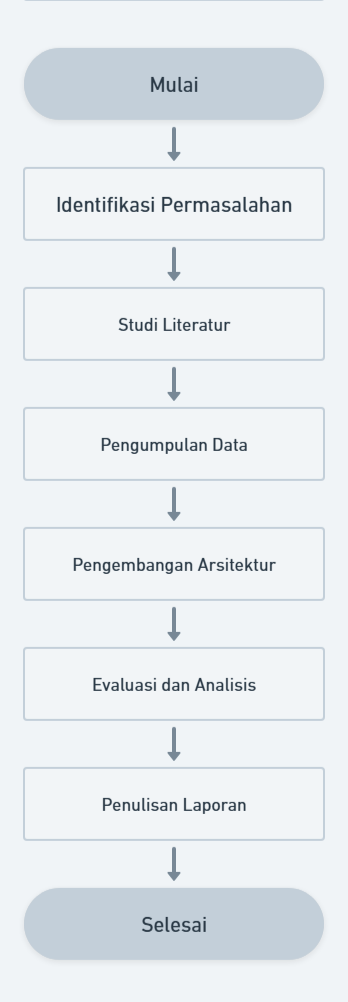
\includegraphics[width=0.3\textwidth]{images/alur-penelitian.png}
	\caption{
		Alur Penelitian
	}
	\label{fig:research-flow}
\end{figure}

Pelaksanaan penelitian ini akan mengikuti suatu alur yang terdiri dari beberapa tahapan utama yang saling terkait dan berurutan,
namun juga memungkinkan adanya iterasi pada beberapa fase tertentu, terutama pada tahap pengembangan dan evaluasi model.
Visualisasi alur penelitian ini disajikan dalam Gambar \ref{fig:research-flow}.
Tahapan-tahapan fundamental tersebut secara terperinci adalah sebagai berikut.


\subsection{Identifikasi Masalah}
Tahap awal ini merupakan fondasi dari keseluruhan penelitian. Proses ini dimulai dengan identifikasi masalah umum mengenai adanya kesenjangan akses terhadap informasi kesehatan mental yang akurat dan terstruktur di Indonesia.
Dari masalah umum tersebut, dirumuskan masalah teknis yang spesifik: bagaimana teknologi RAG dapat dioptimalkan untuk mengatasi tantangan ini.
Identifikasi masalah mencakup analisis kelemahan RAG berbasis vektor standar, yang cenderung kesulitan dalam melakukan penalaran atas hubungan kompleks.
Berdasarkan analisis ini, diajukan hipotesis bahwa penggunaan \textit{Knowledge Graph} dapat memberikan konteks yang lebih kaya dan terstruktur.
Tahapan ini menghasilkan rumusan masalah utama yang berfokus pada optimalisasi ekstraksi pengetahuan untuk membangun KG yang konsisten dan optimalisasi pengambilan pengetahuan dari KG untuk menjawab kueri pengguna secara akurat.

\subsection{Studi Literatur}
Studi literatur dilakukan secara sistematis, komprehensif, dan berkelanjutan.
Hal tersebut bertujuan membangun landasan teoritis yang kokoh, memahami tren dan perkembangan terkini \textit{state-of-the-art} dalam bidang terkait, mengidentifikasi celah penelitian (\textit{research gap}) yang dapat diisi, serta mempelajari berbagai metode dan alat bantu yang relevan.
Proses ini melibatkan pencarian, pengumpulan, analisis, dan sintesis informasi dari berbagai sumber ilmiah jurnal internasional seperti IEEE, ArXiv, JMIR, dll.
Fokus utama area studi literatur meliputi aplikasi teknologi AI pada kesehatan mental, RAG dan \textit{Knowledge Graph}.
Setelah itu, dilakukan analisis mendalam mengenai metode \textit{Knowledge Extraction} dan \textit{Knowledge Retrieval} yang digunakan.

\subsection{Pengumpulan Data}
Pemilihan sumber data didasarkan pada serangkaian kriteria validasi yang telah ditetapkan demi menjaga kualitas sumber pengetahuan.
Kriteria ini bertujuan untuk menyaring informasi dan memastikan hanya konten yang berkualitas tinggi yang akan diintegrasikan ke dalam sistem.
Prinsip utama pemilihan data meliputi kredibilitas dan otoritas lembaga penyusun serta relevansinya terhadap isu kesehatan mental.
Sumber data harus berasal dari lembaga atau institusi yang memiliki otoritas dan rekam jejak yang diakui secara nasional dalam bidang kesehatan dan psikologi, seperti Kementerian Kesehatan, universitas, psikolog, dan lembaga lain.
Selain itu, konten yang terkandung harus relevan dengan permasalah kesehatan mental yang ada, berikut dengan fasilitas yang tersedia, pencegahan, edukasi, dsb.
Mengingat target implementasi sistem ini adalah untuk civitas akademika UGM, maka prioritas diberikan pada sumber data yang tidak hanya relevan untuk konteks kesehatan mental secara umum, tetapi juga spesifik dan dekat dengan lingkungan UGM.
Penggunaan sumber internal ini bertujuan untuk meningkatkan kepercayaan, kedekatan, dan relevansi informasi bagi pengguna akhir.

Berdasarkan kriteria yang ditetapkan, korpus data untuk penelitian ini dikumpulkan dari beberapa sumber, antara lain:

\begin{enumerate}
	\item \textbf{Kementerian Kesehatan (Kemenkes) RI}: Dokumen yang dipublikasikan oleh Kemenkes digunakan sebagai pedoman dasar yang berlaku secara nasional, memberikan pengetahuan mengengai kesehatan mental secara umum di Indonesia.
	\item \textbf{\textit{Center for Public Mental Health} (CPMH) Fakultas Psikologi UGM}: Sebagai pusat studi kesehatan mental, publikasi dari CPMH tidak hanya valid secara akademis, tetapi juga sangat relevan bagi civitas akademika UGM.
	\item \textbf{\textit{Health Promoting University} (HPU) UGM}: Materi dari HPU UGM dipilih karena secara spesifik dirancang untuk mempromosikan kesehatan di lingkungan kampus UGM. Informasi dari sumber ini, seperti mengenai layanan dukungan yang tersedia di UGM, akan sangat praktis dan langsung dapat dimanfaatkan oleh pengguna.
\end{enumerate}

Data yang terkumpul akan melalui proses kurasi untuk memastikan kesesuaian konten dan konsistensi informasi.
Setelah divalidasi, data kemudian akan melalui tahap prapemrosesan untuk membersihkan teks dan menyiapkannya untuk fase pengembangan arsitektur.

\subsection{Pengembangan Arsitektur Ekstraksi dan Penyerapan Pengetahuan}

\begin{figure}[H]
	\centering
	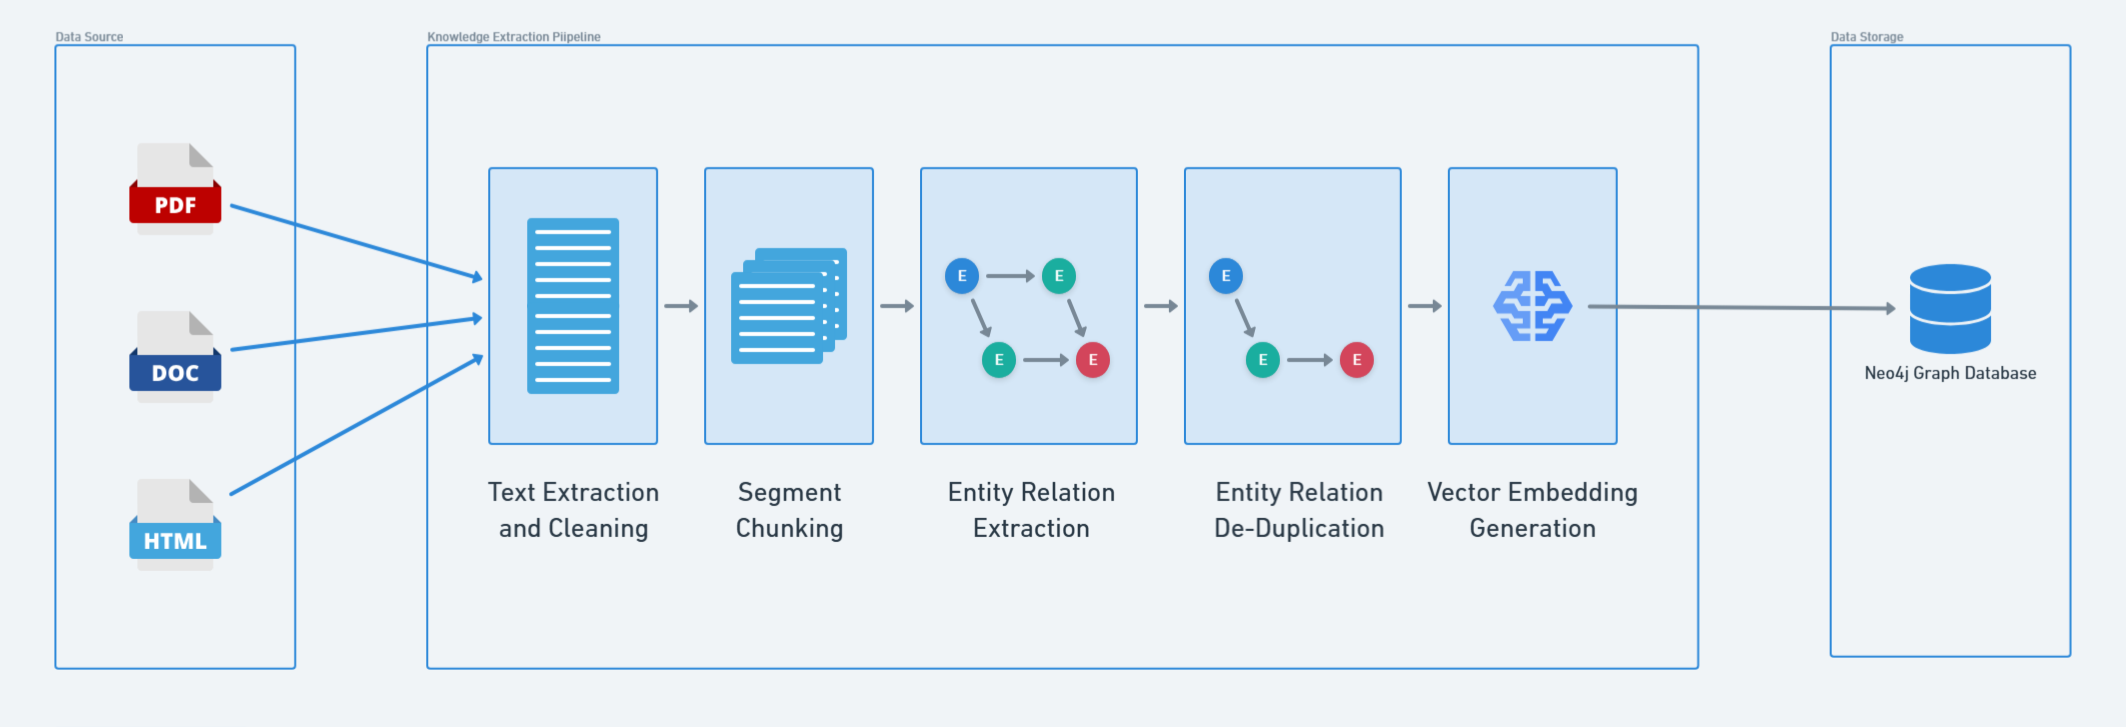
\includegraphics[width=1\textwidth]{images/knowledge-extraction-flow.png}
	\caption{
		\textit{knowledge extraction pipeline}
	}
	\label{fig:knowledge-extraction-pipeline}
\end{figure}

Pengembangan model akan berfokus pada optimalisasi dua komponen krusial pada RAG berbasis \textit{Knowledge Graph}, yaitu \textit{Knowledge Extraction} dan \textit{Knowledge Retrieval}.
Tahap ini bertujuan untuk membangun \textit{Knowledge Graph} yang bersih, konsisten, dan kaya informasi dari berbagai sumber data yang mayoritas tidak terstruktur seperti PDF, DOCX, dan situs web.
Proses ekstraksi pengetahuan diimplementasikan melalui sebuah \textit{pipeline} seperti pada Gambar \ref{fig:knowledge-extraction-pipeline}.
Berikut merupakan penjelasan detail setiap langkah dalam \textit{pipeline}.

\subsubsection{Ekstraksi Teks dari Dokumen}
Hampir semua \textit{language model} dapat memahami informasi dalam bentuk teks.
Untuk itu, langkah awal membangun sebuah \textit{Knowledge Graph} adalah mengekstrak teks mentah dari berbagai sumber data.
Banyak data memiliki format, baik ekstensi, maupun struktur yang beragam karena berasal dari banyak sumber.
Setiap tipe dokumen memiliki cara mengekstraknya masing-masing, misalnya dokumen HTML dapat dikenali strukturnya melalui tagar HTML seperti \texttt{<h1>} untuk menyatakan judul dan \texttt{<p>} untuk menyatakan paragraf.
Dokumen bertipe DOCX terdiri dari kumpulan \textit{file} ZIP yang harus diekstrak untuk mengambil isi dokumen.
Setiap dokumen tersebut juga memiliki struktur penulisan yang tidak seragam, seperti pada dokumen HTML belum tentu mengandung tagar \textit{headline} (\texttt{<h1>}, \texttt{<h2>}, sampai \texttt{<h6>}) untuk menulis, melainkan memakai tagar \texttt{<div>}.
Ketakseragaman format tersebut menjadi tantangan tersendiri dalam mengekstrak teks dari dokumen yang beragam.

Dokumen yang digunakan dalam membangun KG meliputi.
\begin{enumerate}
	\item Buku "Petunjuk Teknis Pencegahan dan Pengendalian Gangguan Mental Emosional" dari Kementerian Kesehatan.
	\item Buku "Panduan Kesehatan Jiwa pada Masa Pandemi COVID-19" dari Kementerian Kesehatan.
	\item Buku "Panduan Pertolongan Pertama Psikologis Pada Upaya Bunuh Diri" dari CPMH.
	\item Artikel dari situs web CPMH
	\item Artikel dari situs web HPU UGM
\end{enumerate}

Sebagian besar dokumen tersebut berada dalam format PDF, sedangkan artikel dari situs web CPMH dan HPU UGM berada dalam format HTML.
Mengekstrak \textit{file} PDF dengan mempertahankan struktur dokumen cukup sulit untuk dilakukan secara langsung karena PDF merupakan tipe dokumen berbasis halaman (\textit{page}) yang mengabaikan struktur keseluruhan seperti judul, paragraf, atau tabel.
Informasi mengenai struktur dokumen penting dijaga untuk langkah selanjutnya.
Untuk itu, dilakukan strategi konversi \textit{file} PDF ke dalam bentuk dokumen yang lebih terstruktur seperti DOCX dan HTML.
Konversi dilakukan menggunakan layanan konversi file online \href{https://www.freeconvert.com/}{FreeConvert}.
Setelah dilakukan konversi dokumen PDF menjadi DOCX barulah isi dari dokumen dapat diambil.
Ekstraksi teks mentah dari dokumen dilakukan menggunakan pustaka python-docx dengan mengambil semua teks yang ada beserta dengan tabel.
Sementara itu, dokumen artikel dari situs web CPMH dan HPU UGM berformat HTML, sehingga proses ekstraksinya lebih sederhana.
Ekstraksi dari HTML lebih mudah karena format ini sudah memiliki struktur bawaan melalui penggunaan tag.
Misalnya, tag \texttt{<h1>} digunakan untuk judul, \texttt{<p>} untuk paragraf, dan \texttt{<table>} untuk tabel.
Untuk merepresentasikan tabel dalam bentuk teks mentah, digunakan format tabel markdown yang intuitif dan mudah dipahami oleh sebagian besar LLM.

\subsubsection{\textit{Structural Chunking}}
Teks yang diekstrak dari dokumen pada langkah selanjutnya akan diekstrak lagi entitas dan relasi yang terkandung di dalamnya.
Ekstraksi entitas dan relasi dilakukan dengan menggunakan LLM.
Namun, LLM modern memiliki ukuran \textit{context window} yang terbatas berkisar ratusan ribu (GPT 4o) hingga 10 juta token (Meta Llama 4 Scout).
Keterbatasan tersebut berimplikasi pada ukuran dokumen (dalam satuan token) menjadi hal yang perlu diperhatikan mengingat sebuah dokumen dapat memiliki ukuran yang besar.
Analisis menggunakan LLM dengan dokumen yang melebihi atau mendekati ukuran maksimal \textit{context window} tidak akan maksimal karena LLM gagal memahami konteks dokumen secara keseluruhan.
Untuk itu, dokumen perlu dipecah menjadi beberapa bagian yang disebut \textit{chunk}.

Proses \textit{chunking} secara umum dapat dilakukan dengan memecah dokumen menjadi beberapa \textit{chunk} dengan panjang tertentu.
Metode \textit{chunking} seperti itu cukup mudah dilakukan, tetapi ada potensi bagian kata atau kalimat dapat terpisah antar \textit{chunk} akibat pemotongan yang menyebabkan kehilangan makna dan konteks.
Dokumen yang masih memiliki informasi strukturnya dapat dimanfaatkan untuk melakukan pemecahan dokumen.
Alih-alih memotong dokumen menjadi potongan berukuran tetap, dokumen dibagi berdasarkan format struktural tertentu, misal dalam dokumen HTML berupa tag \texttt{<h1>} atau pada dokumen DOCX berupa \textit{style paragraph heading} atau \textit{title}.
Pada buku "Petunjuk Teknis Pencegahan dan Pengendalian Gangguan Mental Emosional" yang telah dikonversi menjadi DOCX, dipecah menjadi beberapa chunk berdasarkan judul-judul bagian (seperti BAB I, BAB II, dst).
Pemecahan dokumen berdasarkan judul bagian menghasilkan pecahan dokumen yang memiliki konteks utuh karena pada umumnya setiap bagian dalam dokumen menjelaskan suatu topik bahasan secara utuh.
Hasil dari pemecahan dokumen tersebut yang berjumlah 13 \textit{chunk} kemudian disimpan dalam format TXT untuk kebutuhan \textit{tracing}.
Untuk dokumen yang tidak terlampau panjang tidak akan dipecah, tetapi langsung menjadi 1 bagian dokumen utuh.

\subsubsection{Ekstraksi Entitas dan Relasi}
Ekstraksi entitas dan relasi dalam penelitian ini dilakukan melalui mekanisme inferensi dokumen menggunakan LLM.
Penggunaan LLM untuk mengekstrak entitas dan relasi didasarkan pada kemampuannya dalam memahami struktur dan konteks dokumen yang kompleks dan berukuran besar berkat arsitekturnya yang dilengkapi dengan jumlah parameter yang sangat besar hingga triliunan parameter.
Kapasitas ini memungkinkan LLM untuk menangkap pola linguistik, semantik, dan hubungan antar entitas secara lebih mendalam.
LLM yang digunakan sebagai basis ekstraksi entitas dan relasi adalah Google Gemini 2.5 Flash.
Pemilihan model tersebut didasarkan pada performanya yang sangat baik dan masuk dalam \textit{leaderboard} paling atas pada \href{https://llm-stats.com/}{LLM Stats} setidaknya saat penelitian ini dilakukan dengan skor GPQA (\textit{Graduate-Level Google-Proof Question and Answer}) sebesar 82,8\%.
Faktor krusial lainnya yang tidak kalah penting adalah Gemini 2.5 Flash memiliki ukuran \textit{context window} yang sangat besar hingga 1 juta dibandingkan model LLM lain seperti Claude 3.7 Sonet, Grok-3, dan GPT o3.
Perbandingan performa dan kapasitas LLM tersebut dapat dilihat pada Tabel \ref{tab:llm-comparison}.

\begin{table}[ht]
	\centering
	\caption{Perbandingan performa dan kapasitas LLM modern}
	\label{tab:llm-comparison}
	\begin{tabular}{|l|c|c|}
		\hline
		\textbf{Model}   & \textbf{GPQA} & \textbf{\textit{Context Window}} \\
		\hline \hline
		Gemini 2.5 Flash & 82,8\%        & 1.048.576                        \\
		\hline
		Claude Sonnet 4  & 83,8\%        & 200.000                          \\
		\hline
		OpenAI o3        & 83,3\%        & 200.000                          \\
		\hline
		Grok-3           & 84,6\%        & 128.000                          \\
		\hline
	\end{tabular}
\end{table}

\pagebreak
Setiap \textit{chunk} teks dari dokumen kemudian diproses oleh Gemini 2.5 Flash untuk mengekstrak entitas dan relasi yang terkandung di dalamnya.
Proses ini memanfaatkan teknik \textit{few-shot prompting}, di mana LLM diberikan beberapa contoh konkret untuk memandunya dalam melakukan ekstraksi sesuai dengan ontologi yang telah didefinisikan.
\textit{Prompt} dirancang sejelas mungkin untuk menjelaskan apa yang seharusnya dilakukan oleh LLM dalam proses ekstraksi.
Untuk menjaga jenis entitas yang ditemukan dalam dokumen tidak keluar dari tujuan layanan kesehatan mental maka beberapa istilah yang berkaitan telah didefinisikan terlebih dahulu dalam \textit{prompt}.
Format respons dari LLM juga didefinisikan berupa tipe data JSON yang memudahkan dalam pemrosesan selanjutnya. Format instruksi \textit{prompt} dapat dilihat pada Gambar \ref{fig:prompt-extraction-instruction}.

\begin{figure}[H]
	\centering
	\fbox{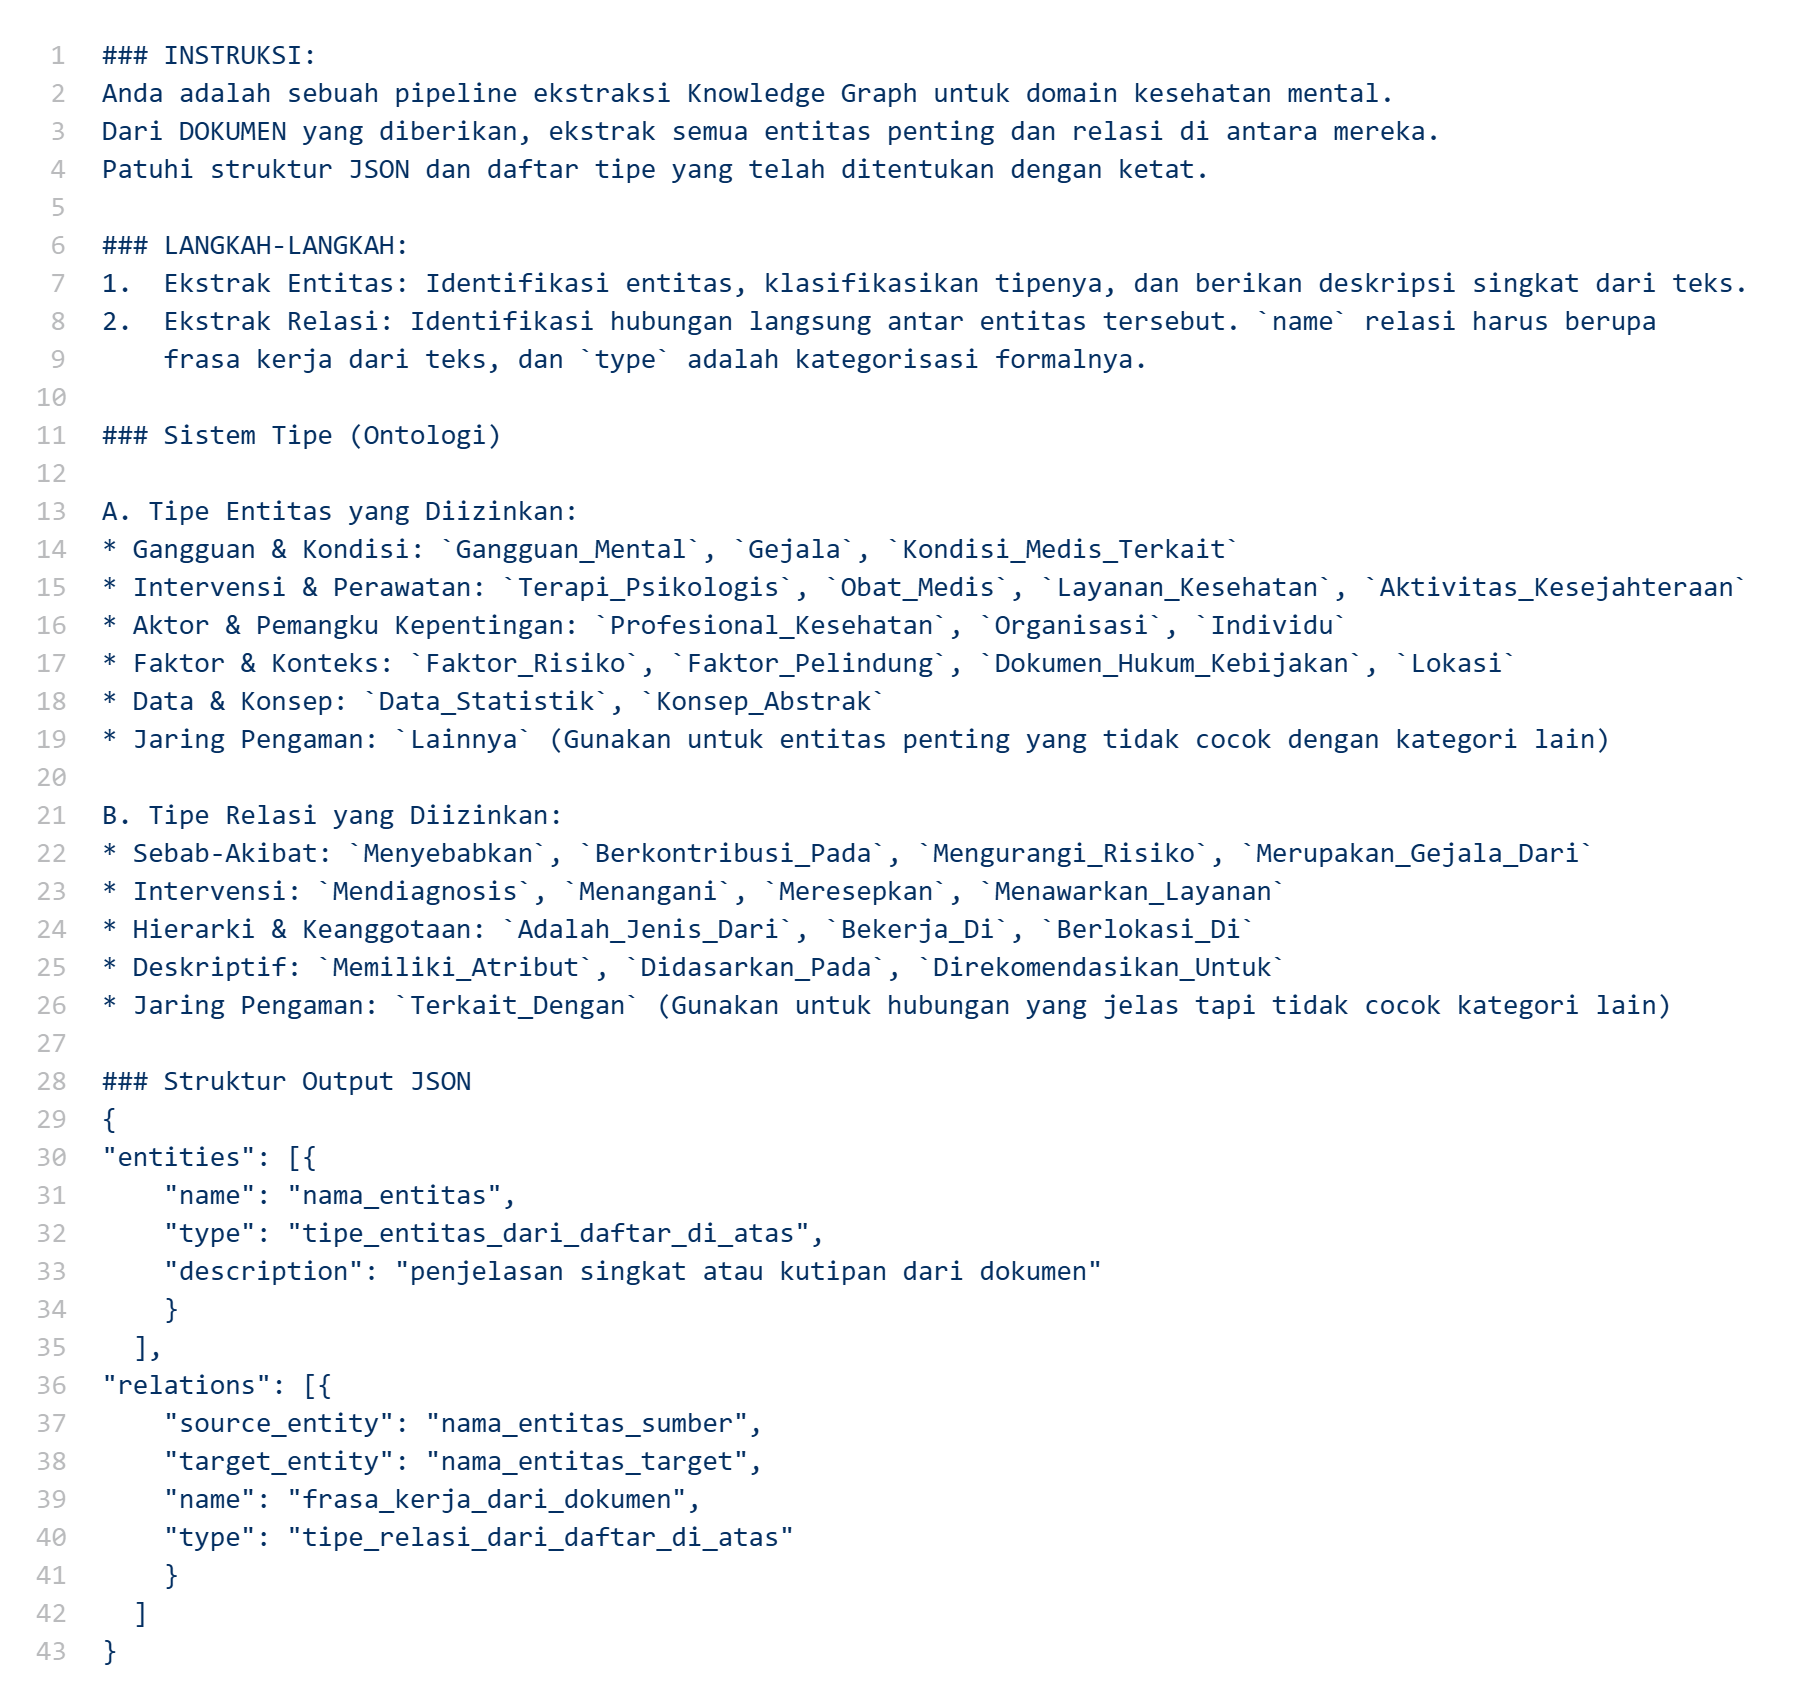
\includegraphics[width=1\textwidth]{images/prompt-extraction-instruction.png}}
	\caption{
		Instruksi LLM untuk melakukan ekstraksi entitas dan relasi
	}
	\label{fig:prompt-extraction-instruction}
\end{figure}

Selain pembatasan istilah dan pemberian instruksi, teknik \textit{few-shot prompting} juga digunakan untuk menghasilkan respons sesuai dengan apa yang diinginkan.
\textit{Few-shot prompting} telah teruji memberikan peningkatan yang signifikan terhadap performa LLM dibandingkan dengan \textit{zero-shot prompting} yang hanya memberikan instruksi saja tanpa contoh \cite{LLMisFewShot2020}.
Teknik ini dilakukan dengan memberikan beberapa contoh (\textit{shot}) input yang akan dihadapi beserta respons yang diharapkan.
Sebuah potongan dari dokumen ditambahkan sebagai contoh input dokumen yang akan diekstrak diikuti dengan keluaran yang diharapkan menggunakan format JSON.
Contoh masukkan dan keluaran pada \textit{prompt} dapat dilihat pada Gambar \ref{fig:prompt-extraction-few-shot}

\begin{figure}[H]
	\centering
	\fbox{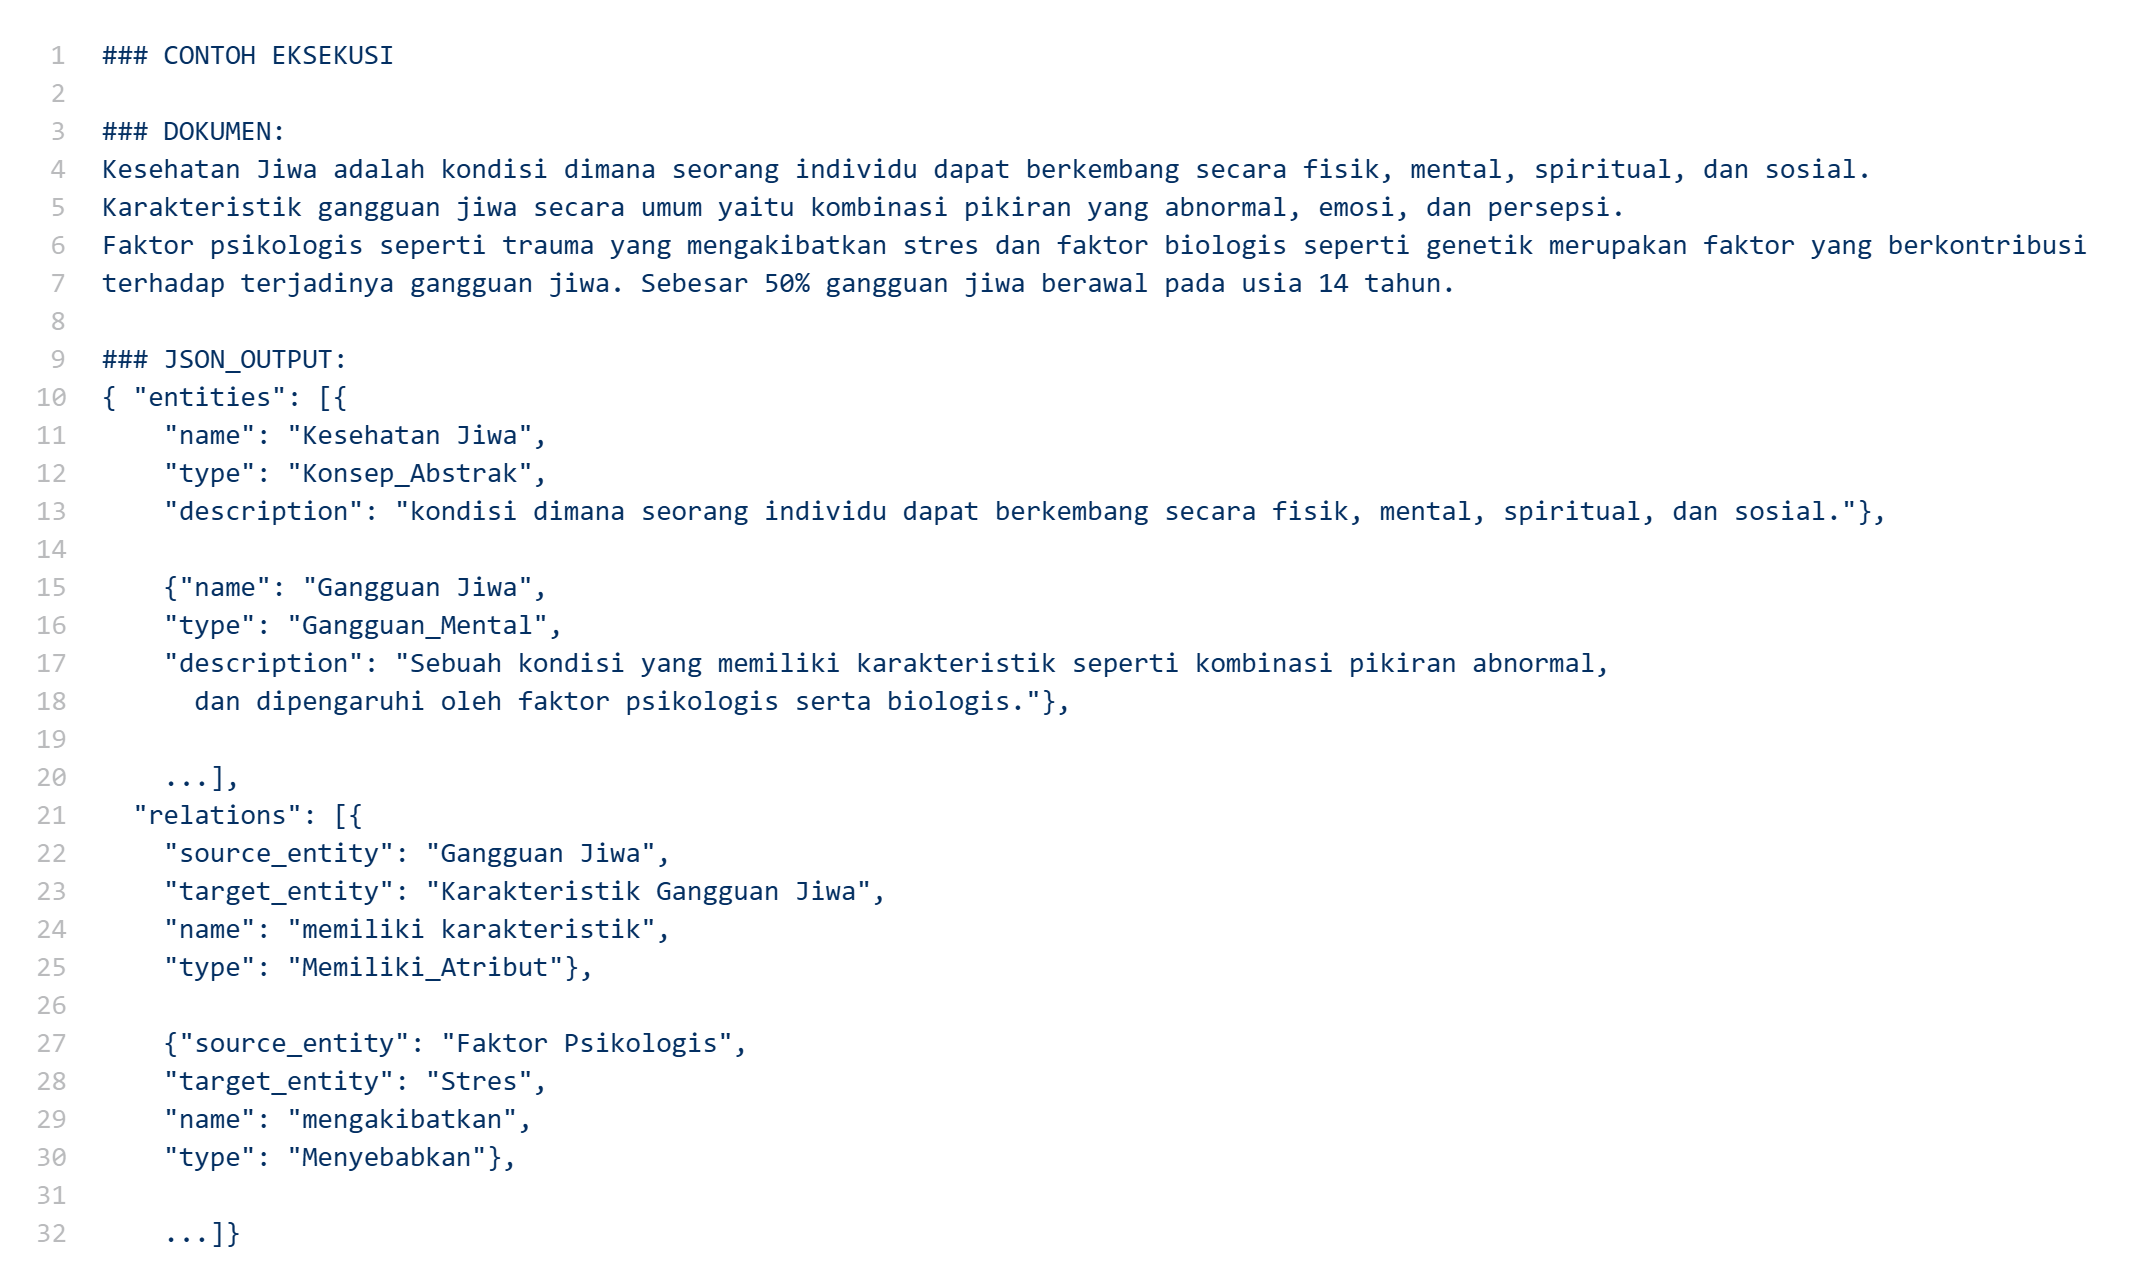
\includegraphics[width=1\textwidth]{images/prompt-extraction-few-shot.png}}
	\caption{
		Penggunaan \textit{few-shot prompting} dengan memberikan potongan dokumen dan keluaran yang diharapkan.
	}
	\label{fig:prompt-extraction-few-shot}
\end{figure}

% \vspace{5cm}
\textit{Prompt} pada Gambar \ref{fig:prompt-extraction-instruction} dan Gambar \ref{fig:prompt-extraction-few-shot} kemudian dieksekusi menggunakan pustaka google genai.
Eksekusi \textit{prompt} diikuti dengan data \textit{chunk} dokumen ditambah dengan konfigurasi struktur JSON yang diinginkan untuk mendapatkan respons bukan dalam bentuk teks, melainkan dalam bentuk JSON yang dapat direpresentasikan dalam bentuk objek pydantic.
Struktur dari respons terbagi menjadi 2 bagian yaitu \texttt{entities} yang berisi daftar entitas dan \texttt{relations} yang berisi daftar relasi.
Setiap entitas memiliki atribut \texttt{name}, \texttt{type}, dan \texttt{description}, sedangkan relasi memiliki atribut \texttt{source\_entity}, \texttt{target\_entity}, \texttt{name}, dan \texttt{type} seperti pada Gambar \ref{fig:entity-relation-structure}.

\begin{figure}[H]
	\centering
	\fbox{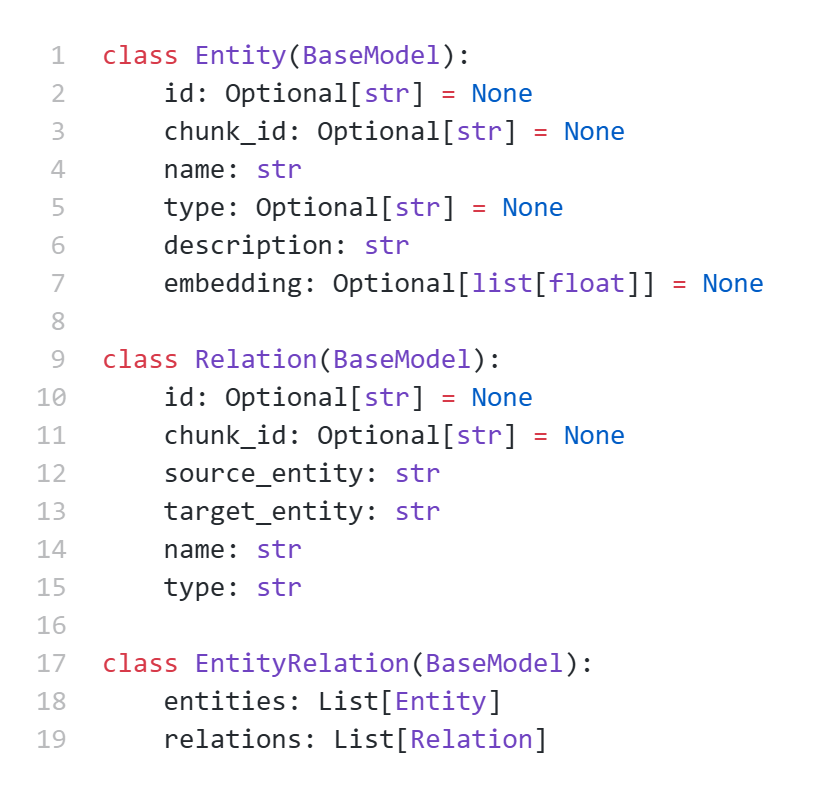
\includegraphics[width=0.5\textwidth]{images/entity-relation-structure.png}}
	\caption{
		Struktur entitas dan relasi yang didefinisikan sebagai \textit{objek} pada pustaka Pydantic
	}
	\label{fig:entity-relation-structure}
\end{figure}

Hasil dari eksekusi \textit{prompt} menghasilkan kumpulan entitas dan relasi dengan format persis seperti skema yang didefinisikan sebelumnya.
Gambar \ref{fig:entity-relation-response} menunjukkan entitas dan relasi yang diekstrak dari potongan dokumen pada Gambar \ref{fig:document-mini-chunk-example}.
\begin{figure}[H]
	\centering
	\fbox{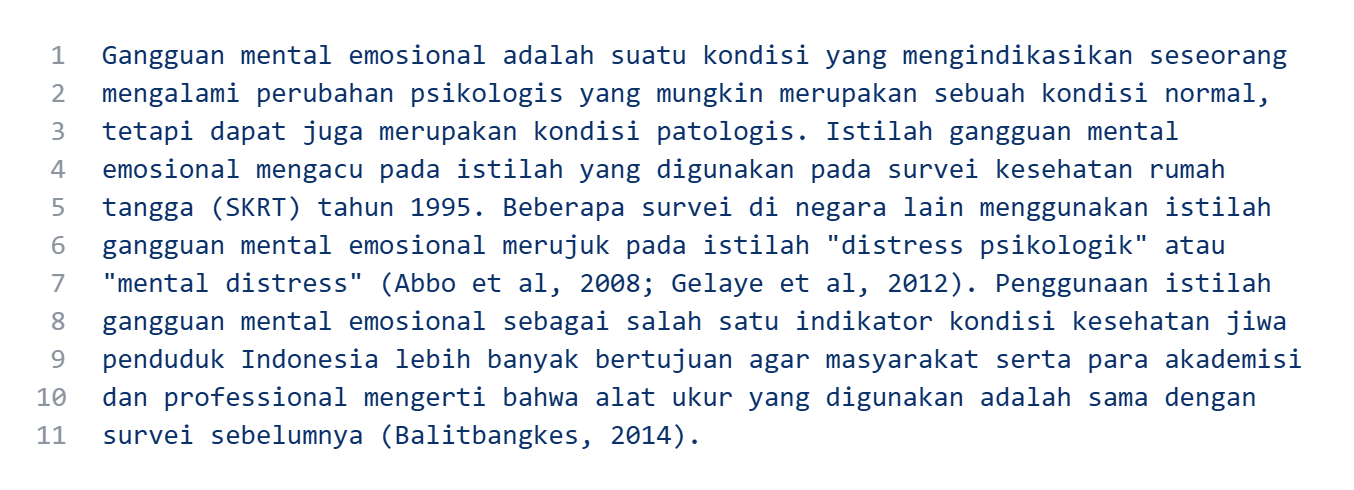
\includegraphics[width=1\textwidth]{images/document-mini-chunk-example.png}}
	\caption{
		Cuplikan dokumen yang diambil dari Buku Petunjuk Teknis Pencegahan dan Pengendalian Gangguan Mental Emosional
	}
	\label{fig:document-mini-chunk-example}
\end{figure}

\begin{figure}[H]
	\centering
	\fbox{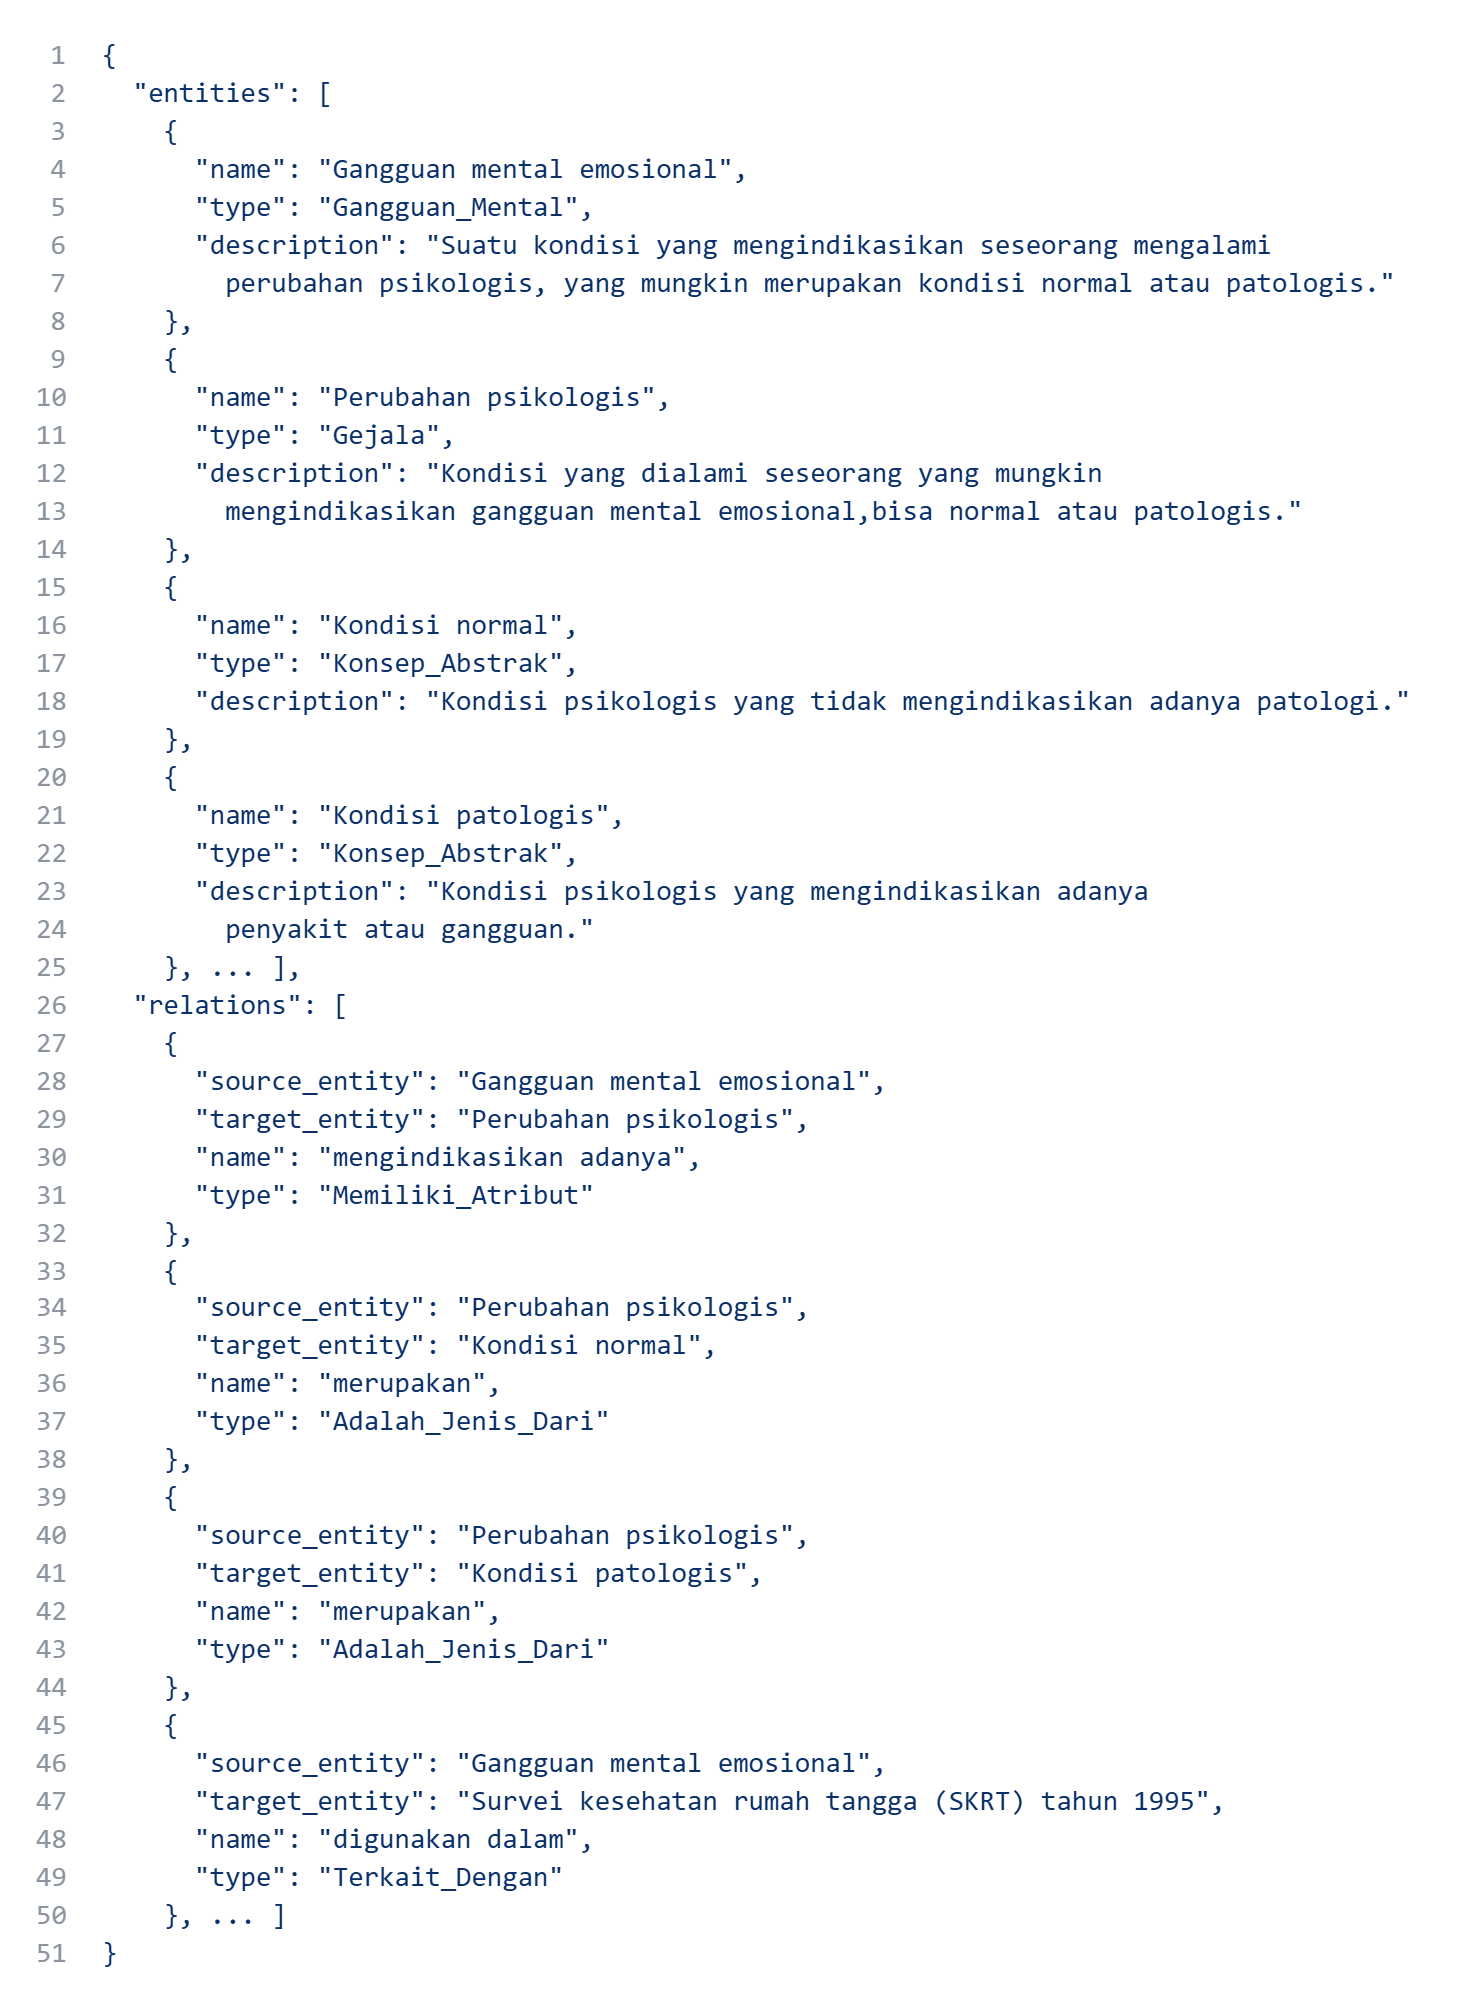
\includegraphics[width=0.8\textwidth]{images/entity-relation-response.png}}
	\caption{
		Respons LLM berupa entitas dan relasi yang diekstrak dari potongan dokumen
	}
	\label{fig:entity-relation-response}
\end{figure}

\subsubsection{Resolusi Entitas dan Relasi}

Hasil dari entitas dan relasi yang telah berhasil diekstrak dari setiap \textit{chunk} kemudian diagregasi dan melalui tahap resolusi untuk memastikan konsistensi.
Entitas dan relasi yang berasal dari \textit{chunk} berbeda mungkin akan memiliki duplikat karena diekstrak secara independen.
Untuk itu, perlu untuk melakukan deduplikasi pada entitas dan relasi guna menghindari redudansi yang tidak perlu.
Entitas yang redundan dapat membuat graf semakin kompleks dan merusak mekanisme \textit{retrieval}.
Deduplikasi dilakukan dengan strategi penggabungan di mana entitas yang memiliki nama yang sama setelah dinormalisasi akan digabungkan menjadi satu.
Untuk mengatasi kehilangan informasi maka deskripsi unik dari entitas duplikat kemudian digabungkan menjadi satu deskripsi utuh.
\textit{Entity mapping} dibentuk saat proses deduplikasi entitas untuk memetakan \texttt{source\_entity} dan \texttt{target\_entity} pada relasi ke entitas yang valid.

\subsubsection{Penambahan Vektor \textit{Embedding}}

Data entitas dan relasi yang disimpan dalam basis data secara umum adalah kumpulan teks yang cukup intuitif bagi manusia untuk memahaminya.
Meskipun demikian, komputer tidak dapat secara langsung "memahami" makna dari tiap-tiap entitas dan relasi.
Bagi manusia mungkin akan mudah untuk mencari entitas dengan nama atau deskripsi yang berkaitan dengan kata kunci atau pertanyaan pengguna.
Untuk itu, diperlukan sebuah representasi tertentu dari data yang dapat dengan mudah dipahami maknanya oleh komputer.
Salah satu representasi data yang cukup mudah diolah oleh komputer sekaligus dapat menangkap makna semantik dari data adalah vektor \textit{embedding}.
Vektor \textit{embedding} merupakan sebuah vektor berdimensi tinggi yang umum digunakan untuk menangkap makna dari sebuah data.
Data dalam bentuk vektor memiliki keuntungan dalam melakukan pencarian semantik (\textit{semantic search}) dengan hanya melakukan operasi \textit{dot product} 2 vektor dapat mengetahui tingkat kemiripan antara 2 data.

Dalam penelitian ini, objek yang akan dilakukan pencarian semantik dalam prosen \textit{knowledge retrieval} adalah entitas.
Untuk itu, setiap entitas akan memiliki representasi vektornya masing-masing.
Vektor \textit{embedding} akan dibentuk menggunakan model gemini-embedding-001.
Model \textit{embedding} ini dipilih menjadi model \textit{embedding} karena memiliki performa yang sangat baik dalam tugas \textit{Semantic Text Similarity} (STS) sebesar 79,40 poin.
Selain itu, model ini juga memiliki kemampuan memahami teks dalam bahasa Indonesia paling baik (67,00 poin) dibandingkan dengan model-model lain \cite{enevoldsen2025MMTEBmassivemultilingualtextEmbeddingModelComp}.
Perbandingan model \textit{embedding} dapat dilihat pada Tabel \ref{tab:embedding-model-comparison}.

\begin{table}[h]
	\centering
	\caption{Perbandingan model \textit{embedding} dalam tugas \textit{Semantic Text Similarity} (STS) dan klasifikasi dalam bahasa Indonesia \cite{enevoldsen2025MMTEBmassivemultilingualtextEmbeddingModelComp}}
	\label{tab:embedding-model-comparison}
	\begin{tabular}{|l|c|c|}
		\hline
		\textbf{Model}       & \textbf{IndoneisanIdClickbaitClassification} & \textbf{{STS}} \\
		\hline \hline
		gemini-embedding-001 & 67,00                                        & 79,40          \\
		\hline
		Qwen3-Embedding-8B   & 65,07                                        & 81.08          \\
		\hline
		Qwen3-Embedding-0,6B & 64,77                                        & 76,17          \\
		\hline
		Qwen3-Embedding-4B   & 64,29                                        & 80,86          \\
		\hline
		voyage-multiligual-2 & 63,23                                        & 68,58          \\
		\hline
	\end{tabular}
\end{table}

Data yang digunakan untuk membuat vektor \textit{embedding} berasal dari gabungan nama, tipe, dan deskripsi dari setiap entitas.
Proses pembuatannya dilakukan secara berulang dengan 100 entitas setiap satu kali pemanggilan API gemini-embedding-001.
Pemanggilan tersebut menghasilkan sebuah vektor dengan 768 dimensi untuk setiap entitas.
Hasil yang berupa vektor tersebut kemudian digabungkan dengan entitas yang bersesuaian dengan atribut \texttt{embedding}.

\subsubsection{Pemuatan Data ke Penyimpanan Basis Data Berbasis Graf}
Entitas dan relasi yang telah dilengkapi dengan vektor \textit{embedding} kemudian dimuat ke dalam basis data graf.
Basis data graf yang dipilih adalah Neo4j karena kemampuannya dalam menyimpan dan menavigasi struktur relasi antar entitas secara efisien, serta mendukung kueri berbasis graf melalui bahasa Cypher.
Neo4j juga mendukung algoritma pencarian berbasis vektor seperti \textit{Approximate Nearest Neighbor} (ANN) secara \textit{native} dengan menerapkan algoritma \textit{Hierarchical Navigable Small World} (HNSW).
Dukungan ini menjadi krusial untuk memungkinkan pencarian semantik dijalankan secara optimal.
Selain itu, Neo4j merupakan sistem basis data yang telah matang dan banyak digunakan, sehingga memiliki dukungan komunitas yang kuat. Dalam pemodelan data, setiap entitas direpresentasikan sebagai \textit{node} dengan atribut seperti \texttt{name}, \texttt{type}, dan \texttt{embedding}, sementara relasi dimodelkan sebagai \textit{edge} yang menghubungkan dua \textit{nodes} dan memiliki atribut seperti \texttt{source\_entity}, \texttt{target\_entity}, \texttt{name}, dan \texttt{type}.
Proses pemuatan data ke Neo4j dilakukan dengan melakukan inisialisasi koneksi ke server, lalu menyusun kueri untuk menambahkan \textit{node} dan \textit{edge} sesuai skema.
Untuk menghindari duplikasi \textit{node}, digunakan pendekatan \texttt{MERGE} dalam Cypher, sehingga entitas dengan identitas yang sama tidak dibuat ulang seperti pada Gambar \ref{fig:cypher-insert-entities}.
Proses ini juga mempertimbangkan efisiensi, khususnya ketika jumlah entitas dan relasi sangat besar, dengan menerapkan strategi \textit{batch insert}.
Dengan memanfaatkan basis data graf, relasi antar entitas dapat ditelusuri secara lebih fleksibel dan intuitif.
Hal ini juga mendukung berbagai analisis struktur data seperti pencarian pola hubungan, pengukuran kedekatan antar \textit{node}, hingga identifikasi komunitas dalam graf.

\begin{figure}[H]
	\centering
	\fbox{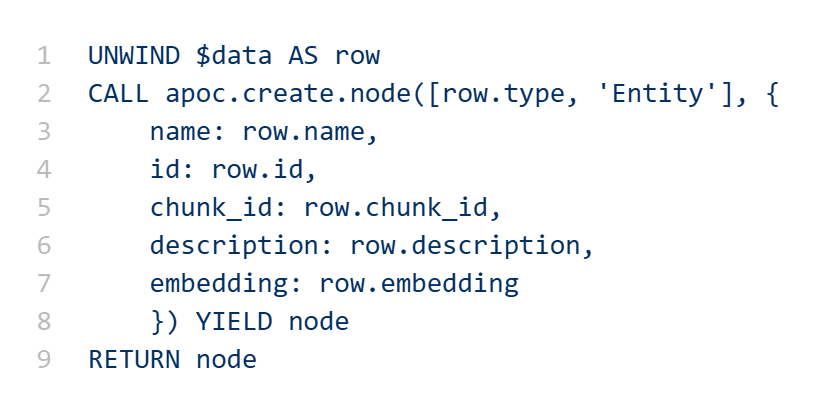
\includegraphics[width=0.8\textwidth]{images/cypher-insert-entities.png}}
	\caption{
		Kode Cypher untuk pemuatan entitas yang berupa \textit{nodes} di basis data Neo4j.
	}
	\label{fig:cypher-insert-entities}
\end{figure}

\subsection{Pengembangan Arsitektur Pengambilan Pengetahuan}
Pengambilan Pengetahuan (\textit{Knowledge Retrieval}) merupakan proses penting dalam sistem berbasis pengetahuan yang bertujuan untuk memberikan jawaban yang relevan berdasarkan pertanyaan pengguna.
\textit{Pipeline} pengambilan pengetahuan yang dikembangkan memiliki beberapa komponen utama seperti klasifikasi kueri, pencarian semantik berbasis vektor dan kata kunci, penelusuran struktur graf, serta konstruksi pengetahuan seperti pada Gambar \ref{fig:knowledge-retrieval-pipeline}.
Setiap komponen ini berkontribusi terhadap ketepatan dan relevansi hasil yang diberikan oleh sistem.

\begin{figure}[h]
	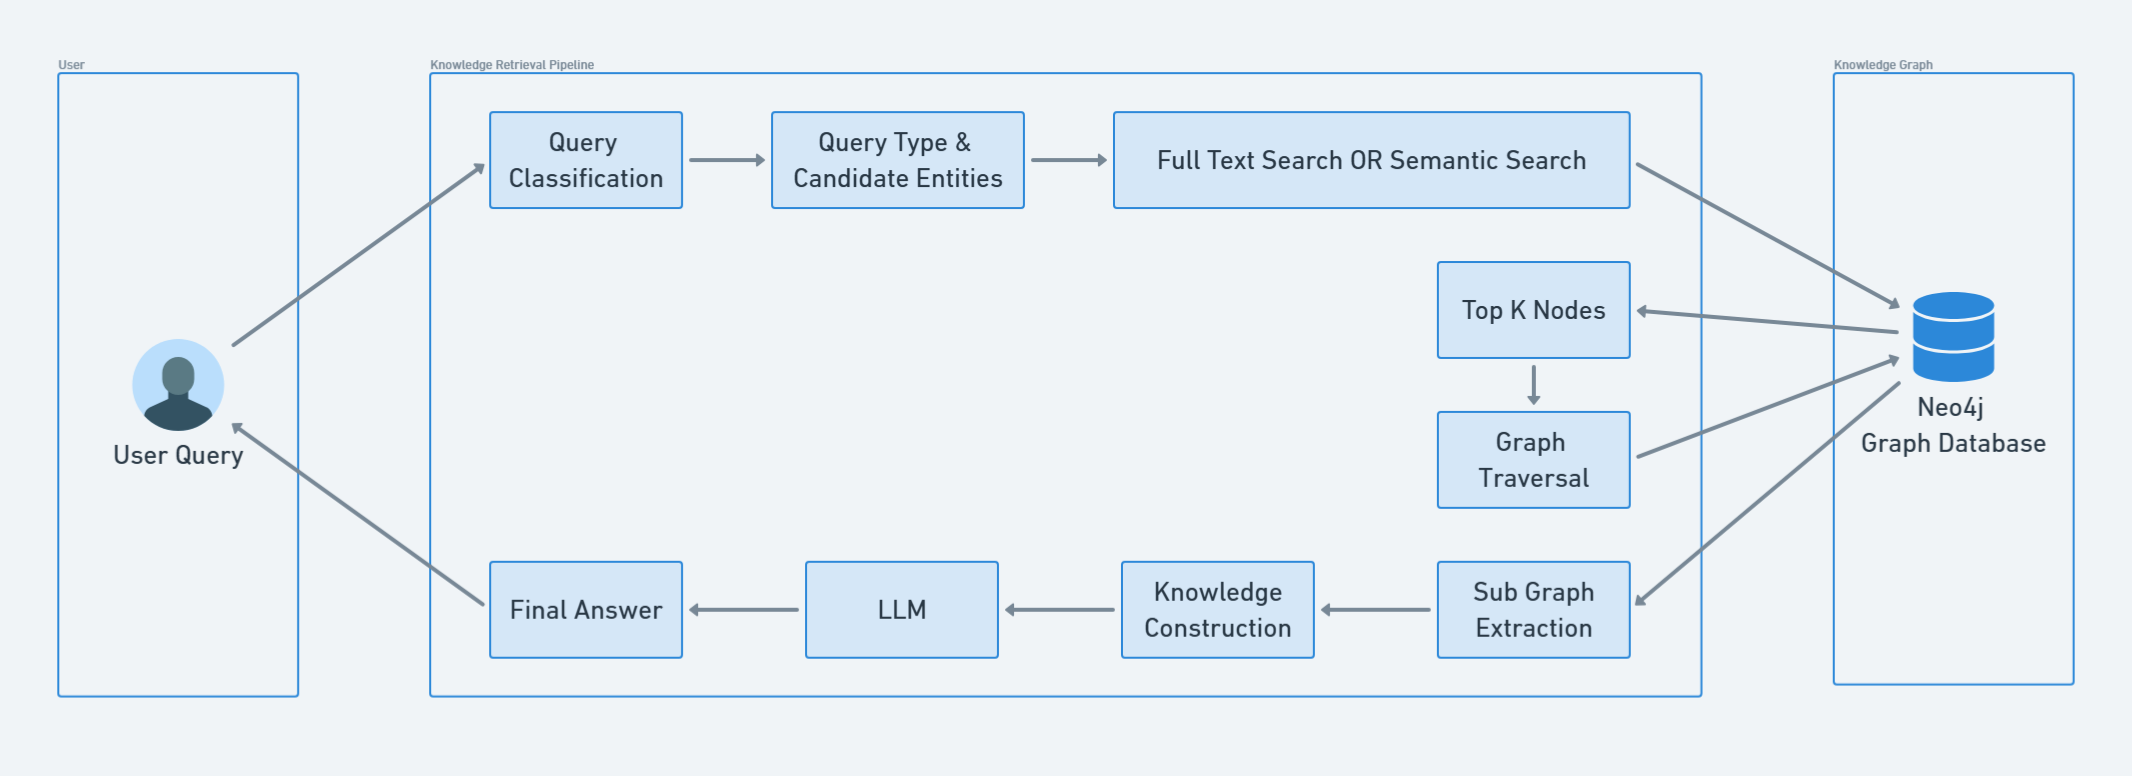
\includegraphics[width=1\textwidth]{images/knowledge-retrieval-pipeline.png}
	\caption{\textit{Pipeline Knowledge Retrieval}.}
	\label{fig:knowledge-retrieval-pipeline}
\end{figure}

\subsubsection{Klasifikasi Kueri dan Ekstraksi Entitas}
Langkah pertama dalam pengambilan pengetahuan adalah klasifikasi kueri terhadap input pengguna.
Proses ini bertujuan untuk mengidentifikasi intensi semantik dari kueri, yang nantinya akan dijadikan sebagai variabel penentu strategi pencarian dalam \textit{Knowledge Graph} yang paling sesuai.
Kueri akan diklasifikasikan menjadi dua kategori seperti pada Tabel \ref{tab:query-classification}

\begin{table}[H]
	\centering
	\caption{Klasifikasi kueri menjadi dua kategori, yaitu \texttt{entity\_query} dan \texttt{path\_query}}
	\label{tab:query-classification}
	\begin{tabular}{|l|p{8cm}|}
		\hline
		\textbf{Kategori}      & \textbf{Keterangan}                                               \\
		\hline
		\texttt{entity\_query} &
		Jenis kueri yang berfokus pada satu entitas utama dan bertujuan untuk mendeskripsikan, mengambil atribut, atau memahami konsep dari entitas tersebut.
		Kueri ini biasanya mengandung permintaan informasi faktual atau deskriptif.                \\
		\hline
		\texttt{path\_query}   &
		Jenis kueri yang melibatkan dua atau lebih entitas, dan bertujuan untuk menelusuri hubungan atau alur keterkaitan antar entitas dalam graf.
		Kueri ini dapat digunakan untuk menemukan relasi eksplisit maupun implisit antara entitas. \\
		\hline
	\end{tabular}
\end{table}

Klasifikasi kueri ini sangat berkaitan dengan strategi pencarian yang akan dilakukan pada basis data graf.
Sebuah kueri diklasifikasikan sebagai \texttt{entity\_query} jika intensi utamanya adalah untuk mendeskripsikan atau melihat lebih detail pada satu atau beberapa konsep sentral.
Pertanyaan dari pengguna seperti \textit{"Apa itu kesehatan mental?"} atau \textit{"Di manakah pusat layanan kesehatan mental di UGM?"} termasuk dalam kategori ini karena memiliki intensi untuk tahu lebih dalam pada suatu konsep yaitu
Untuk menjawab pertanyaan tersebut, sistem hanya perlu menemukan \textit{node} \textit{"Kesehatan Mental"} dan \textit{"Pusat Layanan Kesehatan Mental UGM"} di dalam graf dan mengambil informasi yang melekat langsung padanya (deskripsi) beserta tetangga-tetangga terdekat yang berfungsi sebagai atribut.
Penelusuran ini bersifat melebar dari satu atau beberapa titik pusat.

Sebuah kueri diklasifikasikan sebagai \texttt{path\_query} apabila intensi utamanya adalah memahami relasi, interaksi, atau alur proses antara dua atau lebih konsep yang berbeda.
Pertanyaan dari pengguna seperti \textit{"Bagaimana terapi kognitif Perilaku membantu mengatasi gangguan kecemasan?"} dan \textit{"Apakah stres dapat mengakibatkan penyakit jantung?"}.
Untuk menjawab pertanyaan tersebut, sistem tidak bisa hanya melihat masing-masing \textit{nodes} dan tetangganya.
Sistem harus bisa menemukan hubungan antara beberapa \textit{nodes} lalu menelusuri jalur (\textit{path}) yang menghubungkannya.

Klasifikasi kueri memiliki peran krusial untuk menentukan bagaimana sistem akan melakukan pencarian dalam basis data graf.
Tidak seperti basis data relasional atau basis data lain yang memiliki skema terdefinisi, basis data graf dapat memiliki objek (\textit{node}) yang saling terhubung satu sama lain tanpa terikat pada skema tertentu.
Pencarian yang buruk tidak akan menghasilkan informasi yang tepat sasaran terhadap kueri pengguna.
Untuk itu strategi pencarian menjadi hal yang signifikan terhadap kualitas pengambilan pengetahuan.

Selain klasifikasi kueri, sistem akan mengekstraksi kandidat entitas yang terkandung dalam kueri.
Proses ini bertujuan untuk mengidentifikasi elemen-elemen penting dalam kueri yang berpotensi merujuk pada \textit{node} dalam basis data graf.
Ekstraksi entitas ini penting dilakukan untuk memberikan petunjuk saat melakukan pencarian dalam basis data graf.
Kandidat entitas yang berasal dari kueri pengguna akan dijadikan sebagai kata kunci dalam melakukan pencarian di samping pencarian berbasis vektor.

Proses klasifikasi kueri dan ekstraksi entitas dilakukan secara simultan menggunakan pendekatan berbasis LLM, yang mampu memahami konteks linguistik untuk mengidentifikasi istilah seperti nama penyakit, gejala, proses, atau entitas lainnya.
\textit{Prompt} disusun dengan memberikan instruksi, definisi, dan format keluaran yang diharapkan.
Selain itu, \textit{few-shot prompt} digunakan untuk memberikan contoh input dan keluaran yang diharapkan pada LLM untuk mendapatkan respons yang diinginkan seperti pada Gambar \ref{fig:prompt-query-classification-entity-extraction}.

\begin{figure}[H]
	\fbox{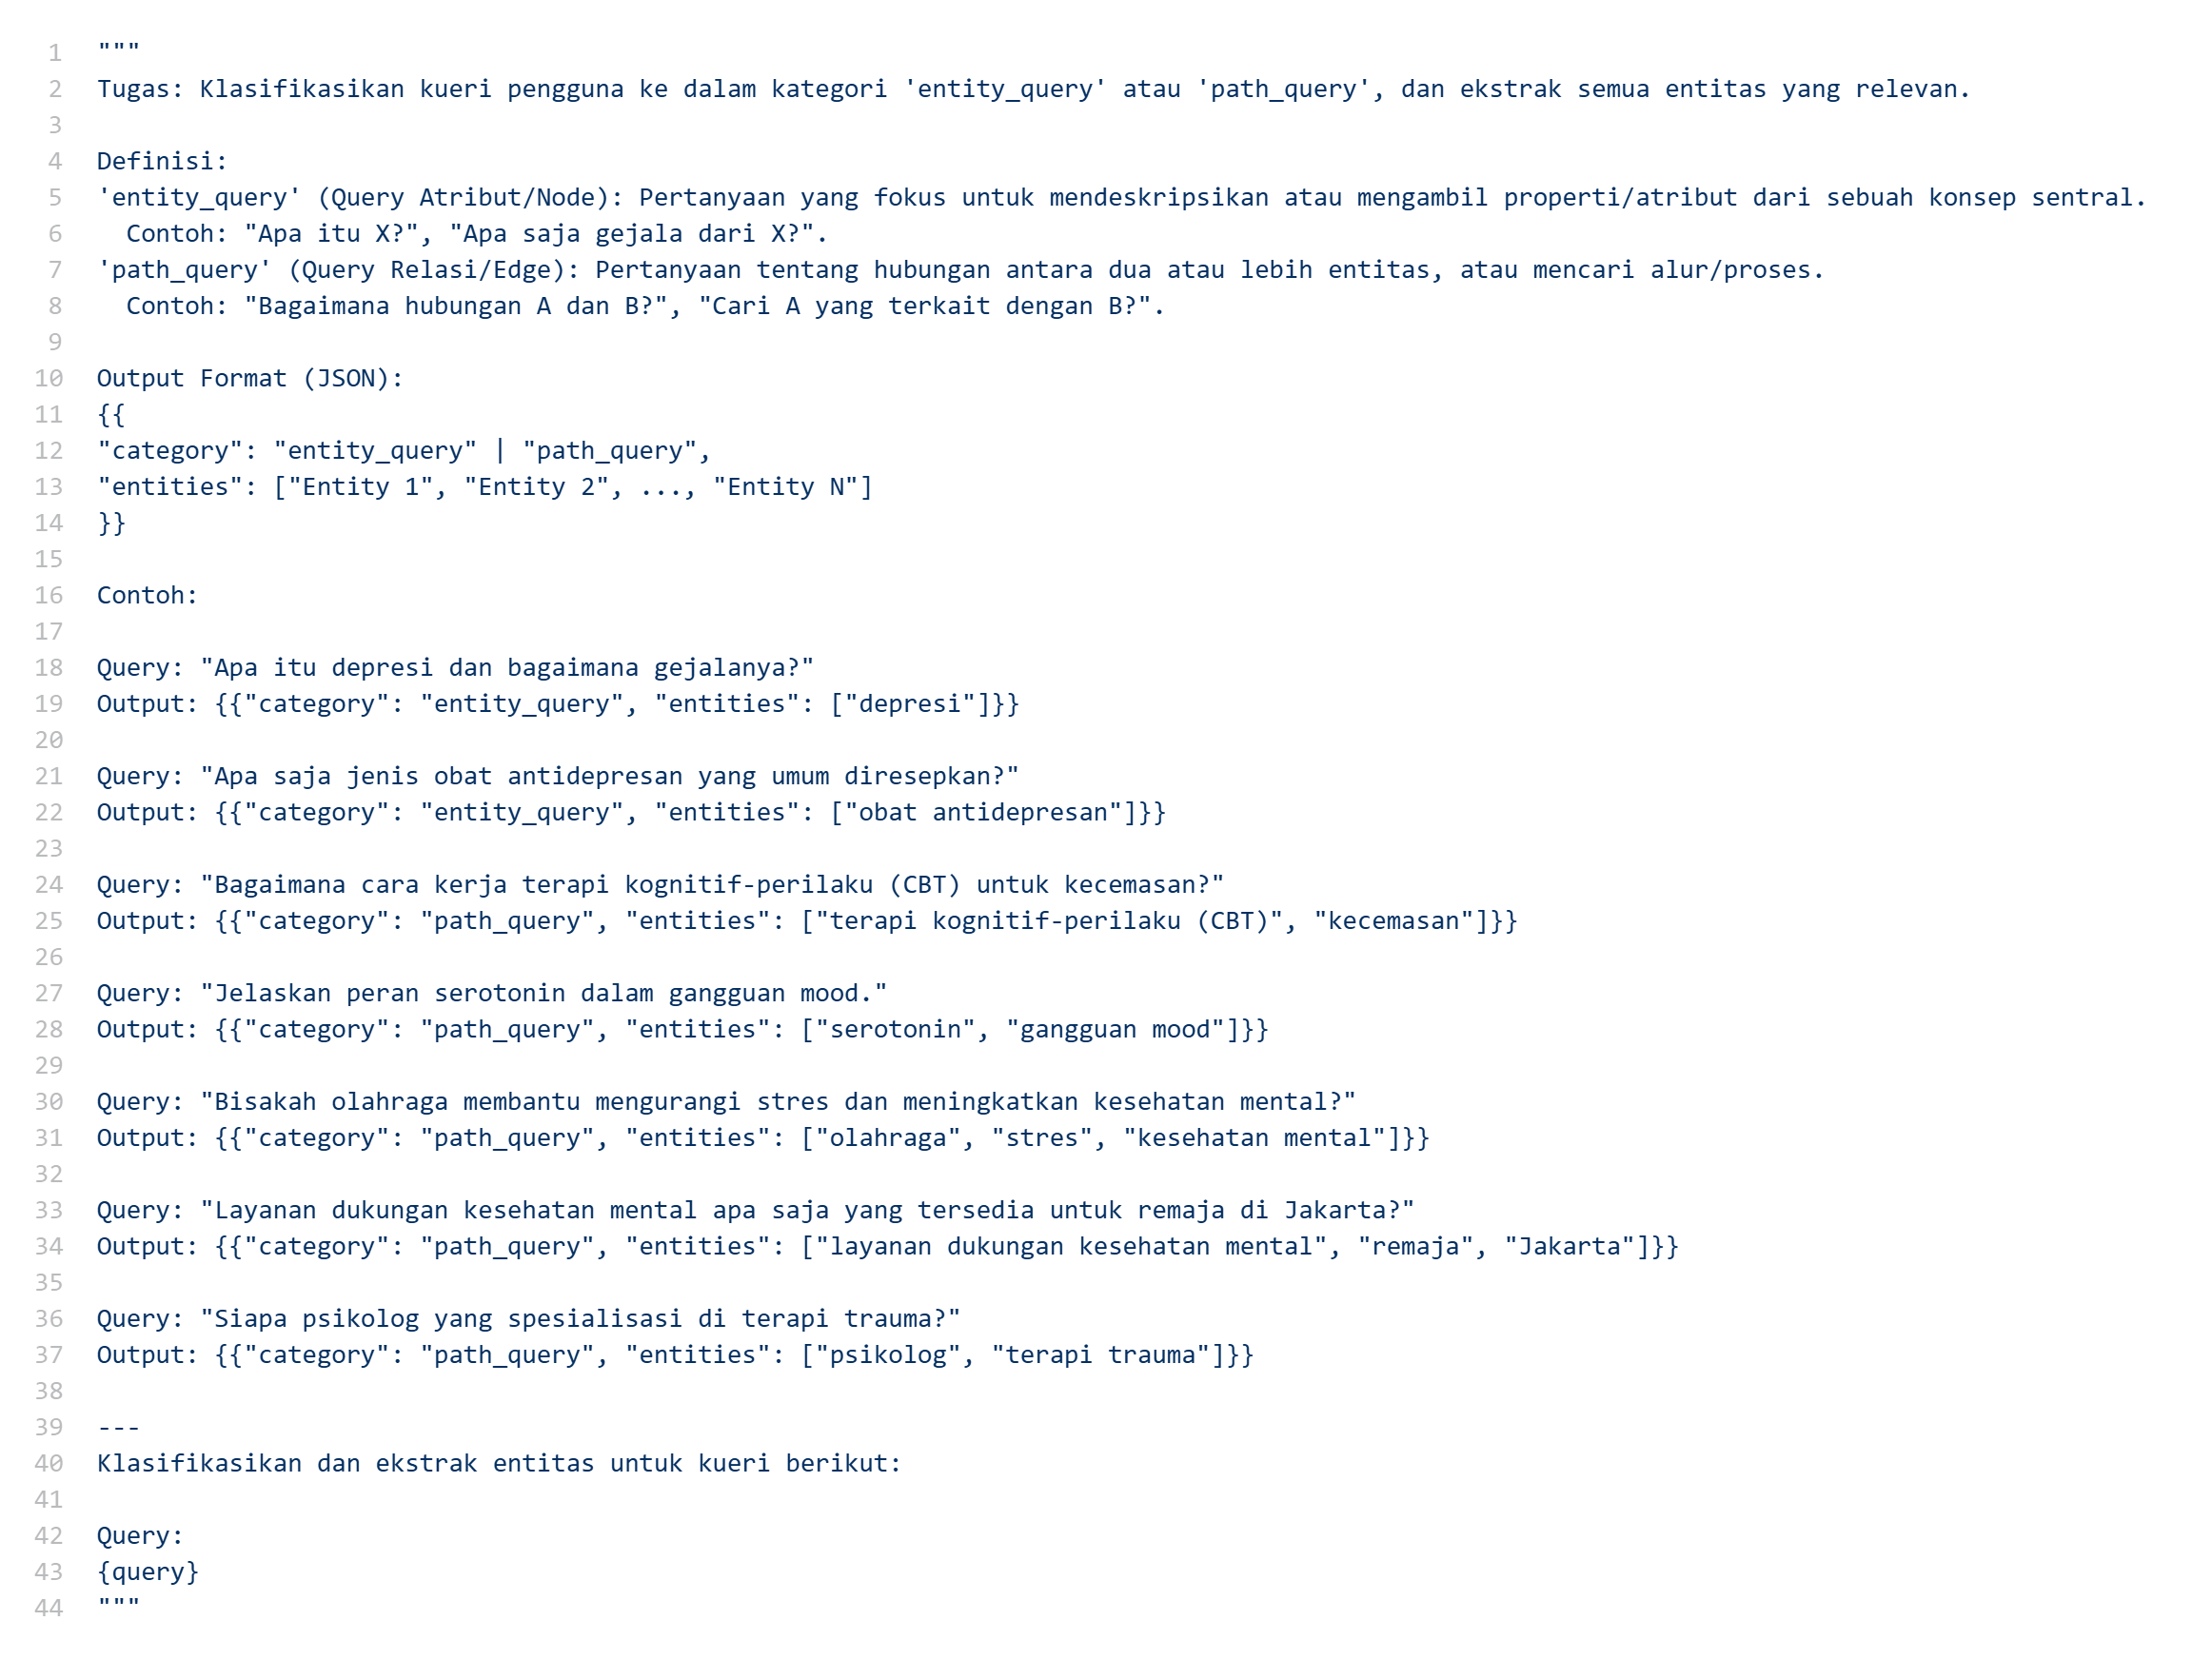
\includegraphics[width=1\textwidth]{images/prompt-query-classification-entity-extraction.png}}
	\caption{\textit{Prompt} yang digunakan untuk memberikan instruksi LLM dalam tugas klasifikasi kueri dan ekstraksi entitas}
	\label{fig:prompt-query-classification-entity-extraction}
\end{figure}

\subsubsection{\textit{Hybrid Search}}
Setelah diekstrak dari kueri pengguna pada proses sebelumnya, kandidat entitas menjadi basis untuk melakukan pencarian entitas dalam graf.
Proses pencarian ini bertujuan untuk mencari \textit{nodes} pada basis data graf yang berkaitan dengan kueri pengguna.
Pencarian didasarkan pada dua variabel utama, yaitu kandidat entitas yang telah diekstrak pada proses sebelumnya dan kueri pengguna itu sendiri.
Tahap pencarian dalam arsitektur ini menggunakan pendekatan \textit{hybrid search} yang merupakan kombinasi dua strategi pencarian, yaitu \textit{full-text search} dan \textit{semantic search} berbasis vektor.
Kedua metode ini dijalankan secara berurutan dengan strategi \textit{fallback} untuk meningkatkan efektivitas pencarian entitas dalam basis data graf.

Proses dimulai dengan melakukan pencarian entitas menggunakan \textit{full-text search} di Neo4j.
Kata kunci yang digunakan berasal dari hasil ekstraksi entitas kandidat pada tahap sebelumnya.
\textit{Full-text search} memanfaatkan indeks teks untuk mencocokkan nama \textit{node} secara eksplisit dalam basis data graf.
Pendekatan ini efektif untuk kueri yang mengandung istilah eksplisit yang cocok dengan nama entitas.

Apabila pencarian berbasis teks tidak menghasilkan entitas yang relevan, misalnya karena variasi bahasa, sinonim, atau struktur kalimat yang tidak eksplisit, maka sistem akan secara otomatis melakukan \textit{fallback} ke pencarian semantik.
Pada tahap ini, sistem mengubah kueri pengguna menjadi vektor \textit{embedding}, kemudian mencari entitas dengan representasi vektor yang paling mirip menggunakan algoritma \textit{Approximate Nearest Neighbor} (ANN) yang didukung secara \textit{native} di Neo4j, yaitu HNSW (\textit{Hierarchical Navigable Small World}).

Dari kedua metode tersebut, sistem akan memperoleh sejumlah entitas paling relevan, yaitu Top-K entitas, yang kemudian digunakan sebagai titik awal untuk proses penelusuran graf.
Pendekatan \textit{hybrid} ini memungkinkan sistem menangani berbagai variasi bentuk pertanyaan, baik yang eksplisit, maupun implisit, serta meningkatkan cakupan pencarian dalam skenario real yang tidak dapat diprediksi.

\subsubsection{Penelusuran Graf}
Setelah diperoleh dari pencarian pada tahap sebelumnya, entitas dan jenis kueri digunakan untuk melakukan penelusuran graf (\textit{graph traversal}) untuk mengumpulkan informasi kontekstual yang lebih komprehensif dari struktur graf.
Tahap ini bertujuan menghasilkan subgraf yang relevan sebagai dasar bagi penyusunan jawaban oleh sistem.
Penelusuran graf dilakukan dengan strategi yang disesuaikan dengan jenis kueri yaitu \texttt{entity\_query} dan \texttt{path\_query}.
Algoritma n-hop neighbor expansion akan digunakan untuk menelusuri graf pada tipe kueri \texttt{entity\_query}, sedangkan algoritma top k shortest path akan digunakan pada tipe kueri \texttt{path\_query}.
Penjelasan lebih lanjut mengenai dua jenis penelusuran graf terdapat pada Tabel \ref{tab:graph-traversal-strategy}.

\begin{longtable}{|p{0.3\textwidth}|p{0.65\textwidth}|}
	\caption{Klasifikasi kueri menjadi dua kategori, yaitu \texttt{entity\_query} dan \texttt{path\_query}}
	\label{tab:graph-traversal-strategy}                                                                                                                     \\
	\hline
	\textbf{Graph Traversal}          & \textbf{Keterangan}                                                                                                  \\
	\hline \hline
	\endfirsthead

	\hline
	\textbf{Graph Traversal}          & \textbf{Keterangan}                                                                                                  \\
	\hline \hline
	\endhead

	\textbf{N-hop Neighbor Expansion} &
	Untuk kueri bertipe \texttt{entity\_query}, sistem menerapkan metode N-hop \textit{Breadth-First Search} (BFS)-style \textit{Neighbor Expansion} dari \textit{node} pusat.
	Dalam sistem ini, nilai N ditetapkan sebagai 1, sehingga hanya \textit{node} tetangga langsung (\textit{one-hop neighbors}) yang diambil.
	Pendekatan ini efektif untuk menangkap atribut langsung dan relasi langsung dari suatu entitas, seperti definisi, komponen, atau karakteristik.
	Proses ini dilakukan dengan \textit{query} Cypher untuk mengambil semua \textit{node} dan \textit{edge} yang terhubung langsung dengan entitas tersebut. \\
	\hline
	\textbf{Top-K Shortest Paths}     &
	Untuk kueri bertipe \texttt{path\_query}, sistem menggunakan pendekatan Top-K \textit{Shortest Path Traversal}, yaitu menelusuri jalur terpendek antara setiap dua entitas kandidat yang dihasilkan dari proses ekstraksi entitas.
	Jalur ini dihitung berdasarkan jumlah \textit{edge} dalam graf, dengan mempertimbangkan arah dan tipe relasi.
	Pendekatan ini digunakan untuk menemukan hubungan langsung maupun tidak langsung antar entitas, serta mengidentifikasi pola keterkaitan yang bermakna.
	Sistem dapat membatasi pencarian hingga K jalur terpendek untuk menjaga efisiensi dan relevansi hasil.                                                   \\
	\hline
\end{longtable}


\subsubsection{Transformasi Konteks}

Transformasi konteks merupakan tahap penting yang menjembatani antara hasil penelusuran graf dan proses penyusunan jawaban oleh \textit{Large Language Model} (LLM).
Tahap ini bertujuan untuk mengubah representasi subgraf hasil penelusuran yang masih bersifat struktural menjadi format teks naratif yang dapat dipahami oleh LLM secara lebih efektif.

Secara teknis, transformasi dilakukan terhadap hasil kueri Cypher yang dikembalikan dalam bentuk struktur data bersarang (\textit{nested}).
Subgraf ini berisi \textit{nodes} entitas beserta relasi antar entitas, termasuk atribut seperti tipe, label, dan deskripsi.
Untuk memungkinkan LLM memproses informasi ini dengan baik, sistem mengubahnya menjadi representasi tekstual menggunakan format blok entitas beranotasi berbasis Markdown.
Format ini mempertahankan struktur semantik penting, seperti tipe entitas, arah relasi, dan deskripsi yang menyertainya.

Alasan utama transformasi ini diperlukan adalah karena LLM bekerja optimal dengan masukan berbasis teks.
Di samping itu, apabila hasil penelusuran graf digunakan secara langsung, akan banyak \textit{overhead} informasi yang sama sekali tidak diperlukan seperti nama atribut yang justru membebani LLM karena \textit{prompt} yang lebih panjang.
Representasi berbentuk teks yang kaya konteks memungkinkan LLM untuk memahami hubungan antar entitas secara utuh, berbeda dengan daftar kalimat terpisah atau output tabel sederhana.
Dengan struktur yang jelas dan eksplisit, LLM dapat melakukan \textit{reasoning} dan menjawab pertanyaan pengguna secara lebih akurat.

Implementasi dari transformasi konteks ini dilakukan melalui fungsi Python yang secara iteratif memproses hasil Cypher \textit{query} dan mengorganisasikannya ke dalam blok-blok informasi yang terstruktur, mirip dengan format dokumentasi.
Dengan pendekatan ini, subgraf dapat diinterpretasikan oleh LLM sebagai narasi pengetahuan, bukan sekadar data mentah, sehingga meningkatkan relevansi dan presisi jawaban yang dihasilkan.

\subsubsection{Respons Final}
Tahap akhir dari arsitektur pengambilan pengetahuan adalah penyusunan jawaban akhir (\textit{final answer}) yang dikembalikan kepada pengguna.
Pada tahap ini, representasi kontekstual yang telah ditransformasikan dari subgraf sebelumnya diproses oleh LLM untuk membentuk jawaban dalam bentuk teks alami yang informatif, ringkas, dan relevan terhadap kueri pengguna.

LLM digunakan sebagai komponen generatif yang memanfaatkan informasi terstruktur yang telah diformat menjadi teks.
Dengan input yang kaya konteks, termasuk anotasi entitas, deskripsi, dan relasi antar \textit{node}-LLM dapat melakukan \textit{reasoning} semantik untuk menghasilkan jawaban yang tidak hanya berbasis fakta, tetapi juga disampaikan dalam bahasa yang mudah dipahami.

Sistem dapat mengatur gaya dan format jawaban yang dihasilkan, seperti bahasa formal atau santai sesuai kebutuhan aplikasi, panjang jawaban (ringkas vs. naratif), dan penyisipan kutipan entitas atau sumber dari graf, jika diperlukan.
Proses ini dilakukan secara deterministik (menggunakan \textit{prompt engineering} dengan temperatur rendah) untuk memastikan konsistensi dan menghindari halusinasi jawaban yang tidak berdasarkan pada data yang tersedia dalam graf.
Dengan pendekatan ini, sistem tidak hanya berfungsi sebagai pencari informasi (\textit{retriever}), tetapi juga sebagai penyaji pengetahuan yang mampu menyusun informasi menjadi jawaban utuh yang siap dikonsumsi pengguna.

\subsection{Evaluasi dan Analisis}
Tahapan evaluasi dan analisis merupakan fase krusial untuk mengukur performa sistem \textit{Retrieval-Augmented Generation} (RAG) berbasis \textit{Knowledge Graph} yang telah dibangun.
Sistem RAG ini terdiri dari dua komponen utama, yaitu sistem \textit{retrieval} yang bertugas mengambil konteks yang relevan dengan pertanyaan dan sistem \textit{generation} yang menghasilkan respons akhir.
Untuk itu, evaluasi dilakukan pada kedua komponen tersebut.

\subsubsection{Penyiapan \textit{Dataset} Evaluasi}
Salah satu tantangan dalam mengevaluasi sistem RAG adalah ketiadaan \textit{dataset} percakapan yang secara khusus sesuai dengan domain dan karakteristik dokumen yang digunakan.
Tidak seperti metode \textit{fine-tuning} yang sejak awal menggunakan data percakapan, RAG cukup memerlukan dokumennya saja.
Untuk menjawab tantangan tersebut, dilakukan pembuatan \textit{dataset} evaluasi sintesis mandiri yang seolah-olah meniru tanya jawab dengan pengguna.
Pendekatan ini dimaksudkan agar evaluasi cukup akurat mengukur kemampuan sistem dalam menjawab pertanyaan berdasarkan korpus pengetahuan yang telah diindeks.

Data percakapan untuk evaluasi dibuat berdasarkan dokumen yang dipakai untuk membangun \textit{Knowledge Graph} yang berupa potongan-potongan dokumen (\textit{document chunks}).
Setiap potongan dokumen tersebut dianggap sebagai dasar kebenaran (\textit{ground truth}) untuk menghasilkan beberapa \textit{dataset} evaluasi.
Selain potongan dokumen, \textit{Knowledge Graph} juga berperan dalam membentuk \textit{dataset} evaluasi, khususnya untuk evaluasi bagian sistem \textit{retrieval}.

Sistem akan melakukan iterasi pada setiap potongan dokumen yang telah diindeks disertai dengan \textit{nodes} dari subgraf yang berasosiasi sebagai konteks.
Konteks tersebut kemudian dimasukkan ke dalam \textit{Large Language Model} (LLM) dengan instruksi atau \textit{prompt} yang telah dirancang.
\textit{Prompt} tersebut meminta LLM untuk berperan sebagai seorang ahli pembuatan data untuk menghasilkan \textit{dataset} evaluasi yang terdiri dari beberapa \textit{field} seperti pada Tabel \ref{tab:evaluation-dataset-fields}.

\begin{table}[h]
	\centering
	\caption{\textit{Fields} pada \textit{dataset} evaluasi}
	\label{tab:evaluation-dataset-fields}
	\begin{tabular}{|p{0.3\textwidth}|p{0.6\textwidth}|}
		\hline
		\textbf{\textit{Fields}} & \textbf{Keterangan}                                                                                    \\
		\hline
		\texttt{query}           &
		\textit{Query} adalah sebuah pertanyaan yang jawabannya dapat ditemukan dari konteks yang disediakan.                             \\
		\hline
		\texttt{query\_lable}    &
		\textit{Query lable} adalah kategori kueri yang nilainya dapat berupa \textit{entity query} atau \textit{path query}.             \\
		\hline
		\texttt{golden\_nodes}   &
		\textit{Golden nodes} adalah \textit{nodes} yang berasal dari \textit{knowledge graph} yang diperlukan untuk menjawab pertanyaan. \\
		\hline
		\texttt{golden\_answer}  &
		\textit{Golden answer} merupakan jawaban akurat dari kueri dan didasarkan pada konteks yang tersedia.                             \\
		\hline
	\end{tabular}
\end{table}

Selain itu, teknik \textit{few-shot} digunakan pada \textit{prompt} untuk memberikan beberapa contoh data evaluasi yang diharapkan.
Dalam setiap potongan dokumen akan dihasilkan pertanyaan setidaknya setengah dari jumlah \textit{nodes} yang tersedia.
Jumlah tersebut dipilih guna memberikan keleluasaan LLM untuk memberikan variasi pertanyaan dan tidak terpaku bahwa setiap \textit{node} harus memiliki satu pertanyaan.

\textit{Prompt} yang sudah dirancang kemudian dieksekusi dengan model OpenAI \texttt{o4-mini}.
Pemilihan model dari OpenAI didasarkan pada model yang digunakan dalam proses evaluasi harus berbeda dengan model yang digunakan pada operasional.
Hal tersebut dilakukan guna menghindari bias dalam evaluasi apabila model yang sama digunakan dalam menjawab pertanyaan sekaligus evaluasi.
Model OpenAI \texttt{o4-mini} merupakan salah satu model kekinian yang dioptimalkan untuk tugas \textit{reasoning} yang cepat.
Kelebihan tersebut sangat sesuai dengan kebutuhan membuat \textit{dataset} evaluasi berdasarkan instruksi.

\subsubsection{Evaluasi Sistem \textit{Retrieval}}
Evaluasi sistem \textit{retrieval} bertujuan untuk mencari tahu seberapa efektif komponen \textit{retriever} dalam menghasilkan konteks yang bersesuaian.
Konteks memiliki peranan yang krusial bagi komponen generatif dalam menghasilkan jawaban akhir yang memiliki landasan informasi akurat.
Kualitas jawaban akhir yang dihasilkan secara signifikan dipengaruhi oleh relevansi dan kelengkapan konteks yang disediakan.
Apabila \textit{retriever} gagal menemukan konteks yang tepat, maka jawaban akhir akan berisiko tidak akurat bahkan cenderung menghasilkan "halusinasi", yaitu informasi yang tidak didasarkan pada data faktual.
Halusinasi ini menjadi masalah besar terlebih apabila sistem ini akan diterapkan sebagai \textit{chatbot} layanan kesehatan mental yang penggunanya sering berhubungan langsung dengan pasien yang memiliki risiko mental.
Kesalahan informasi dapat mengakibatkan dampak yang fatal baik bagi penderita kesehatan mental ataupun bagi pengguna pada umumnya.

Dalam kasus RAG berbasis \textit{Knowledge Graph}, konteks berarti subgraf yang dihasilkan oleh \textit{retriever}.
Setiap kali sistem menjawab pertanyaan, subgraf yang berkaitan dengan pertanyaan akan diambil dari basis data.
Subgraf tersebut terdiri dari dua komponen yaitu \textit{node} yang berisi informasi entitas dan \textit{edge} yang berupa relasi antar entitas.
Dalam proses evaluasi ini, hanya komponen nama  \textit{node} yang digunakan dengan asumsi bahwa \textit{nodes} yang dihasilkan sudah mewakili konteks informasi.
Hal tersebut dilakukan untuk menyederhanakan evaluasi dengan membandingkan \textit{nodes} yang dihasilkan dengan \textit{golden nodes} pada \textit{dataset} evaluasi sebagai \textit{ground truth}.
Untuk setiap pertanyaan, sistem \textit{retrieval} akan diminta untuk mengambil n subgraf yang relevan dengan pertanyaan.
Bentuk dari subgraf terbagi menjadi dua kategori berdasarkan jenis pertanyaannya, yaitu \textit{neighbor expansion} dan n \textit{shortest path}.
Masing-masing jenis subgraf tersebut memiliki struktur yang berbeda, tetapi tidak menjadi masalah karena hanya diambil nama \textit{nodes} yang terkandung di dalamnya.
\textit{Nodes} tersebut kemudian dibandingkan dengan \textit{golden nodes} untuk menghasilkan sejumlah metrik kuantitatif seperti pada Tabel \ref{tab:retrieval-evaluation-metrics} yang digunakan untuk mengukur efektivitas sistem \textit{retrieval}.

\begin{table}[H]
	\centering
	\caption{Metrik evaluasi sistem \textit{retrieval} }
	\label{tab:retrieval-evaluation-metrics}
	\begin{tabular}{|p{0.2\textwidth}|p{0.7\textwidth}|}
		\hline
		\textbf{Metrik}                              & \textbf{Keterangan}                                                                                                                                                                                                                                    \\
		\hline
		\textbf{\textit{Precision}}                  &
		Presisi mengukur proporsi \textit{nodes} yang relevan di antara \textit{nodes} yang dihasilkan oleh \textit{retriever}. Metrik ini menjawab pertanyaan \textit{"Seberapa banyak dari hasil yang diberikan oleh sistem yang benar-benar berkaitan?"}.                                                  \\
		\hline
		\textbf{\textit{Recall}}                     &
		\textit{Recall} mengukur proporsi \textit{nodes} relevan yang berhasil ditemukan dari semua \textit{nodes} relevan yang tersedia. Metrik ini menjawab pertanyaan \textit{"Seberapa lengkap cakupan hasil yang diberikan oleh sistem?"}.                                                               \\
		\hline
		\textbf{\textit{Hit Ratio}}                  &
		\textit{Hit Ratio} mengukur apakah setidaknya satu \textit{node} yang relevan berada di antara $k$ hasil teratas yang dikembalikan. Ini adalah metrik biner yang hanya peduli apakah jawaban yang benar ada di dalam daftar hasil, tidak peduli di peringkat berapa.                                  \\
		\hline
		\textbf{\textit{Mean Reciprocal Rank} (MRR)} &
		\textit{Mean Reciprocal Rank} (MRR) mengukur seberapa cepat sistem memprioritaskan \textit{nodes} yang relevan. Metrik ini berfokus pada dokumen peringkat dari \textit{node} relevan pertama yang ditemukan. Skor tinggi menunjukkan sistem memprioritaskan \textit{node} relevan di peringkat atas. \\
		\hline
	\end{tabular}
\end{table}

\subsubsection{Evaluasi Respons Akhir}
Evaluasi respons akhir berfokus pada penilaian terhadap kualitas jawaban akhir yang dihasilkan sistem, khususnya pada bagian generatif setelah menerima konteks dari komponen \textit{retrieval}.
Evaluasi ini mempertimbangkan beberapa parameter penting, antara lain faktualitas, relevansi, dan kebenaran jawaban, guna memastikan bahwa respons akhir yang diberikan kepada pengguna memiliki nilai informatif yang tinggi dan sesuai dengan pertanyaan yang diajukan.

Keberhasilan sistem RAG tidak hanya ditentukan oleh kemampuan dalam mengambil konteks yang relevan, tetapi juga oleh kemampuan LLM dalam menghasilkan jawaban yang benar dan relevan berdasarkan konteks tersebut.
Dalam beberapa kasus, bahkan jika konteks yang diambil sudah tepat, model generatif dapat tetap menghasilkan jawaban yang tidak faktual, tidak tepat sasaran, atau terlalu umum.
Oleh karena itu, evaluasi terhadap respons akhir menjadi sangat penting untuk menilai efektivitas akhir sistem RAG secara holistik, mendeteksi adanya halusinasi, dan menjamin bahwa jawaban benar-benar menjawab pertanyaan pengguna secara akurat.

\vspace{1cm}
Evaluasi dilakukan dengan menggunakan \textit{framework} RAGAS (Retrieval-Augmented Generation Assessment), yaitu sebuah kerangka kerja modern dan terstandardisasi yang dirancang khusus untuk mengevaluasi \textit{pipeline} RAG secara menyeluruh.
RAGAS akan menghitung sejumlah metrik evaluasi terhadap jawaban yang dihasilkan dengan membandingkannya terhadap \textit{golden answer} dan konteks. Pendekatan ini memungkinkan evaluasi yang kuantitatif, objektif, dan replikatif.
Metrik yang digunakan untuk menilai kualitas jawaban akhir terdapat pada Tabel \ref{tab:generation-evaluation-metrics}.

\begin{table}[h]
	\centering
	\caption{Metrik evaluasi sistem \textit{Generation} }
	\label{tab:generation-evaluation-metrics}
	\begin{tabular}{|p{0.2\textwidth}|p{0.7\textwidth}|}
		\hline
		\textbf{Metrik}                               & \textbf{Keterangan}                                                                               \\
		\hline
		\textbf{\textit{Faithfulness}}                &
		Mengukur sejauh mana jawaban yang dihasilkan tetap berpegang pada informasi dalam konteks.
		Skor tinggi menunjukkan bahwa jawaban tidak mengandung halusinasi.                                                                                \\
		\hline
		\textbf{\textit{Answe \newline Relevancy}}    &
		Menilai apakah jawaban benar-benar menjawab pertanyaan yang diajukan.
		Jawaban faktual tetapi tidak menjawab pertanyaan secara langsung akan memiliki skor rendah.                                                       \\
		\hline
		\textbf{\textit{Answer \newline Correctness}} &
		Membandingkan jawaban yang dihasilkan dengan \textit{golden answer} untuk mengukur kesesuaian dan kebenaran faktual.
		Ini merupakan indikator langsung dari akurasi jawaban.                                                                                            \\
		\hline
		\textbf{\textit{Answer\newline Similarity}}   &
		Mengukur kemiripan semantik antara jawaban yang dihasilkan dan \textit{golden answer} menggunakan \textit{cosine similarity} atas representasi vektor dari kedua jawaban.
		Skor tinggi menunjukkan bahwa secara makna, jawaban yang dihasilkan sangat mirip dengan \textit{golden answer}, meskipun berbeda secara tekstual. \\
		\hline
	\end{tabular}
\end{table}